\documentclass[a4paper]{article}
%\usepackage{ctex}
\usepackage[colorlinks,linkcolor=black,urlcolor=black]{hyperref}
%---------------------------------------------
%\usepackage[cache=false]{minted} 
%---------------------------------------------
\usepackage{float}
\usepackage{mhchem}
\usepackage{pdfpages}
\usepackage{mathrsfs}
\usepackage{pdfpages}
\usepackage{listings}
\usepackage{cancel}
\usepackage{enumerate}
\usepackage{amsmath}
\usepackage{amssymb}
\usepackage{booktabs}
\usepackage{colortbl}
\usepackage{graphicx}
\usepackage{subfigure}
\usepackage{ulem}
\usepackage{siunitx}
\usepackage{wrapfig}
\usepackage{geometry}
\usepackage{indentfirst}
\usepackage{multirow} 
\setlength{\parindent}{2em}
\renewcommand{\baselinestretch}{1.6}
\usepackage[greek,english]{babel} 
%\renewcommand\thesection{\Roman{section}}
%\renewcommand\thesubsection{\Alph{subsection}}
\geometry{left=2.5cm,right=2.5cm,top=2.5cm,bottom=2.5cm}
\begin{document}
\begin{titlepage}
\begin{figure}[!htbp]
\center

\includegraphics[width=12cm]{ji_logo.png}
\end{figure}
\noindent\rule[0.25\baselineskip]{\textwidth}{1pt}
\begin{center}
\Large{\bfseries  VE401, Probabilistic Methods in Engineering}
\vspace{1cm}

\Huge{\bfseries  Term Project 2:}\\
\Huge{\bfseries Police Shootings in the United States}

\vspace{1.5cm}

\Large SP2019  Group 17\\
\Large \textbf{Group members}\\

\begin{tabular}{l l}
Hou Yichun & 517370910128\\
Ma Ziqiao & 517370910114\\
Shen Dinghao & 517370910200\\
Wang Zibo & 516021910050\\
Yang Zhe & 517021911127\\
\end{tabular}

\vspace{1cm}
\Large \textbf{Instructed by}\\
\Large Dr. Horst Hohberger\\

\vspace{1cm}
{\bfseries \today}\\
\vspace{1cm}

UM-SJTU Joint Institute
\end{center}
\end{titlepage}
\section{Abstract}
David Spiegelhalter and Arthur Barnett's \textit{London Murder} analyses murder cases in London between 2004 and 2007. Also, \textit{Washington Post} provides a database recording the occurrence of fatal police shootings. \textit{Washington Post} claims that there have been 270 citizen killed by police shooting since 2019, as of March $15^{th}$.

In this project, we are going to use data above, applying mathematical methods we obtained in ve401, to do some data analysis. We will summarize the data sources and conclude how the term "fatal police shooting" is used here. We will use \textit{Mathematica} to create a histogram of numbers of fatal police shooting from 2015 to 2018. We will test the hypothesis that the number of police shootings in the US between 2015 and 2018 follows a Poisson distribution. We will test whether there is evidence that the
average number of police shootings depends on the weekday. We will calculate the ($1-\alpha$)-confidence interval of parameter $k$. We will check whether fatal police shooting data between January and March in 2019 follows a Poisson distribution and calculate the value of $k$. We will obtain 95\% prediction intervals for the
number of mass shootings in 2019 based on the data for 2015 to 2018, and plot the result.

\paragraph{Key Words}
Fatal police shootings\quad Poisson distribution\quad Confidence interval\quad Prediction interval\quad Mathematica


\newpage
\tableofcontents
\newpage
\listoffigures
\listoftables
\newpage
\section{Project Introduction}
\subsection{Problem Description}
According to the article \textit{London murders: a predictable pattern?}, published by David Spiegelhalter and Arthur Barnett [1], the pattern of London murders between April 2004 and September 2007 are analyzed based on data of the London Metropolitan Police and figures. 

As to this project, we are required to analyze the pattern of Fatal Police Shootings in the U.S. with the similar statistical method from the article \textit{London murders: a predictable pattern?}[1] as well as an another article \textit{How The Washington Post is examining police shootings in the United States.} [4].

The analysis is based on the data obtained from the Database of Fatal Police Shootings of the Washington Post [6] from January 2015 to April 2019. It includes processing the data, discussion on what kind of distribution the data belongs to, whether the number of police shootings depends on weekdays and confidence interval for the parameter of the distribution and plotting the corresponding figures with Mathematica.

By finding out the pattern of fatal police shooting, we can predict the number of mass shooting in the future, which may be helpful to public safety in the future as mass shooting has become a social issue recently in the United States.

\subsection{Project Objectives}
The project is based on \textit{London murders: a predictable pattern?}, published by David Spiegelhalter and Arthur Barnett [1] and the data obtained from the Database of Fatal Police Shootings of the Washington Post [6].

The objectives of the project are listed below:
\begin{itemize}
\item Give a thorough and introductory summary of the data of ``fatal police shooting''. Plot a Histogram with Mathematica to help the overview of the data.
\item Find out whether the occurrence of police shootings in the United States from years 2015 to 2018 follows a Poisson distribution with Pearson's Chi-squared Goodness-of-Fit Test.
\item Find out whether the occurrence of police shootings depends on the weekday with Goodness-of-Fit Test classified by average number of shooting and exact number of shooting. Plot the corresponding figures with Mathematica.
\item Prove and calculate the confidence interval for Poisson Parameter with the normal approximation to Poisson distribution.
\item Find and give proper estimations and predictions for fatal police shooting numbers based on updated data in 2019. Plot the corresponding figures about prediction interval and observed Data to help discussion.
\end{itemize}


\newpage

\section{Data Analysis}
\subsection{Objectives}
This section is oriented to question i) and ii).

The objectives of this section is give a thorough and introductory analysis of the data which the project bases on. Especially, we are interested in the term ``fatal police shooting'' used to describe the data, and we will represent the overview of data by date a histogram.
\subsection{Definitions and Notations}
\paragraph{Date Histogram} DateHistogram is a histogram which features a horizontal axis of DateObjects. This figure gives a clear view of the number of fatal police shooting in a day within a long range of time [3].

\subsection{Summary of Source of Data}
The following summary cites some factual basis based on \textit{How The Washington Post is examining police shootings in the United States}, officially written by Julie Tate et al [4].
\paragraph{Database Introduction}
The data we research on in the project comes from a database called the Washington Post, which compiles ``a database of every fatal shooting in the United States by a police officer in the line of duty since Jan. 1, 2015''.

\paragraph{Source of Data}
The Washington Post collects the information by culling
\begin{itemize}
\item Local news reports;
\item Llaw enforcement websites;
\item Social media;
\item Monitoring other independent databases, e.g. \textit{Killed by Police} and \textit{Fatal Encounters}.
\end{itemize}

We note that do not use the data logged by the \textit{FBI} and \textit{the Centers for Disease Control and Prevention}, because these databases acknowledge the incompleteness of their data.
\subsection{Key Term Characterization}
The database records only ``Fatal Police Shooting'', because only those shootings in which \textbf{a police officer, in the line of duty, shoots and kills a civilian will be recorded}. The data are in favour of Black Lives Matter movement and police accountability discussion. 

Hence, the Post is not tracking 
\begin{itemize}
\item Deaths of people in police custody and non-shooting deaths (not shooting);
\item Fatal shootings by off-duty officers (not police);
\item Police shootings that did not lead to deaths (not fatal).
\end{itemize}

\subsection{Data Completeness}
The Post's database is updated regularly as fatal shootings are reported and as facts emerge about individual cases on \texttt{GitHub} [6]. Hence, we had access to the \texttt{csv} file recording all fatal police shootings.

However, we noticed that the database on GitHub is updated only to Feb. 14, 2019. For complete data, we refer the the official website of Washington Post, which reports the latest shooting on Apr. 15, 2019 [7].
\subsection{Date Histogram of Fatal Police Shooting}
With the application of \texttt{Mathematica}, we recreate a version of Figure 1 in [1] for the data between Jan. $1^{st}$, 2015 and Dec. $31^{st}$, 2018. The plot is a DateHistogram with a step length of 1 day, and vertical axis representing the number of fatal police shootings in that day (Figure 1).

\begin{figure}[!htbp]
\centering
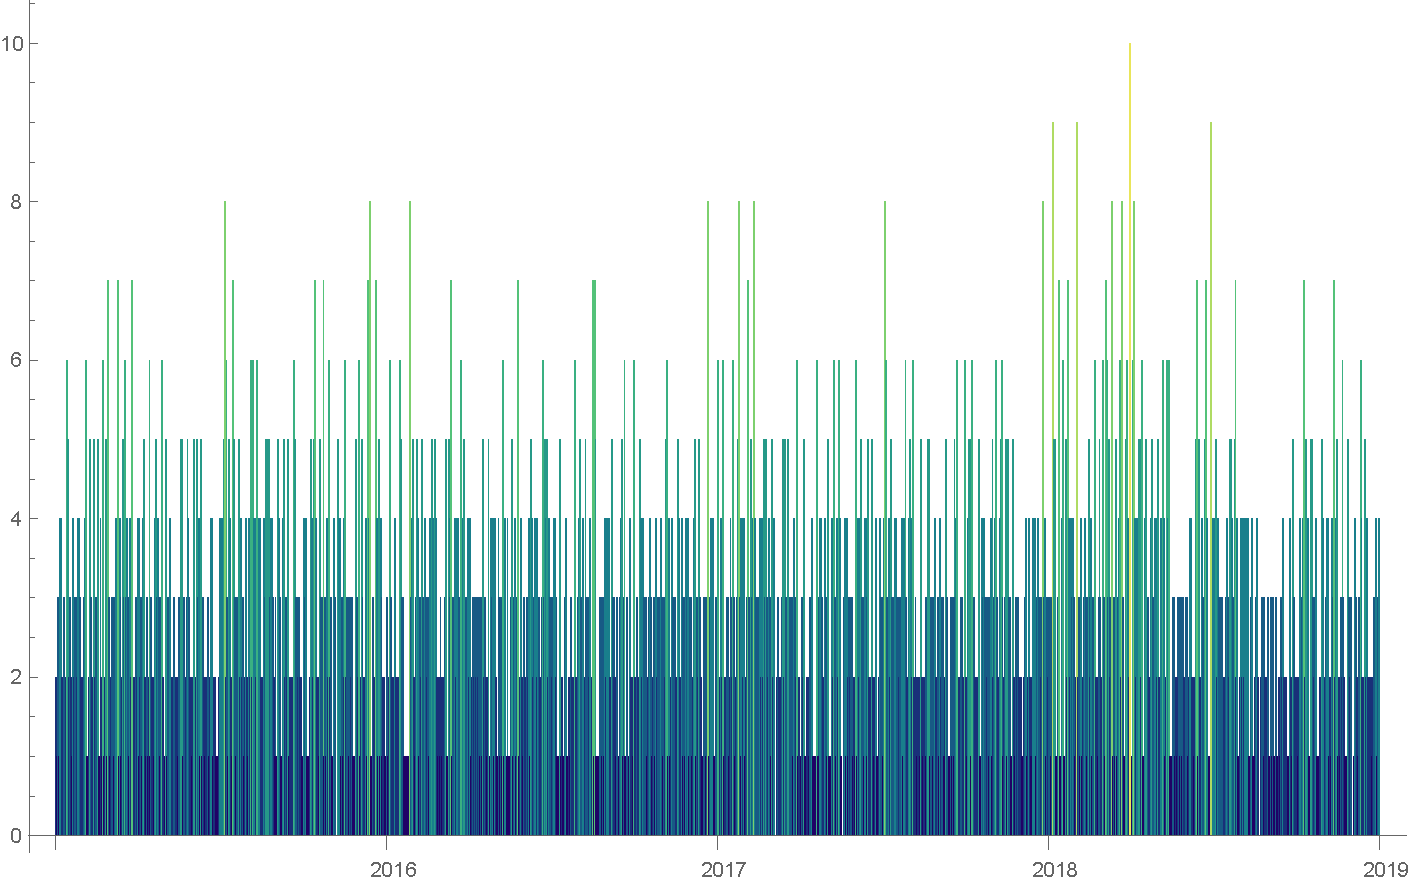
\includegraphics[width=1\linewidth]{ex2.pdf}
\caption{The Histogram of Numbers of Fatal Police Shooting}
\end{figure}

For convenience of observations, we plot the figure in a way that the lighter the color is, the more shoots observed in that day.

\newpage

We noticed that 2016 is a leap year with Feb. $29^{th}$, check the data with command \texttt{Tally}, we observed that there is 1 shooting in Feb. $29^{th}$, 2016 (Figure 2).

\begin{figure}[!htbp]
\centering
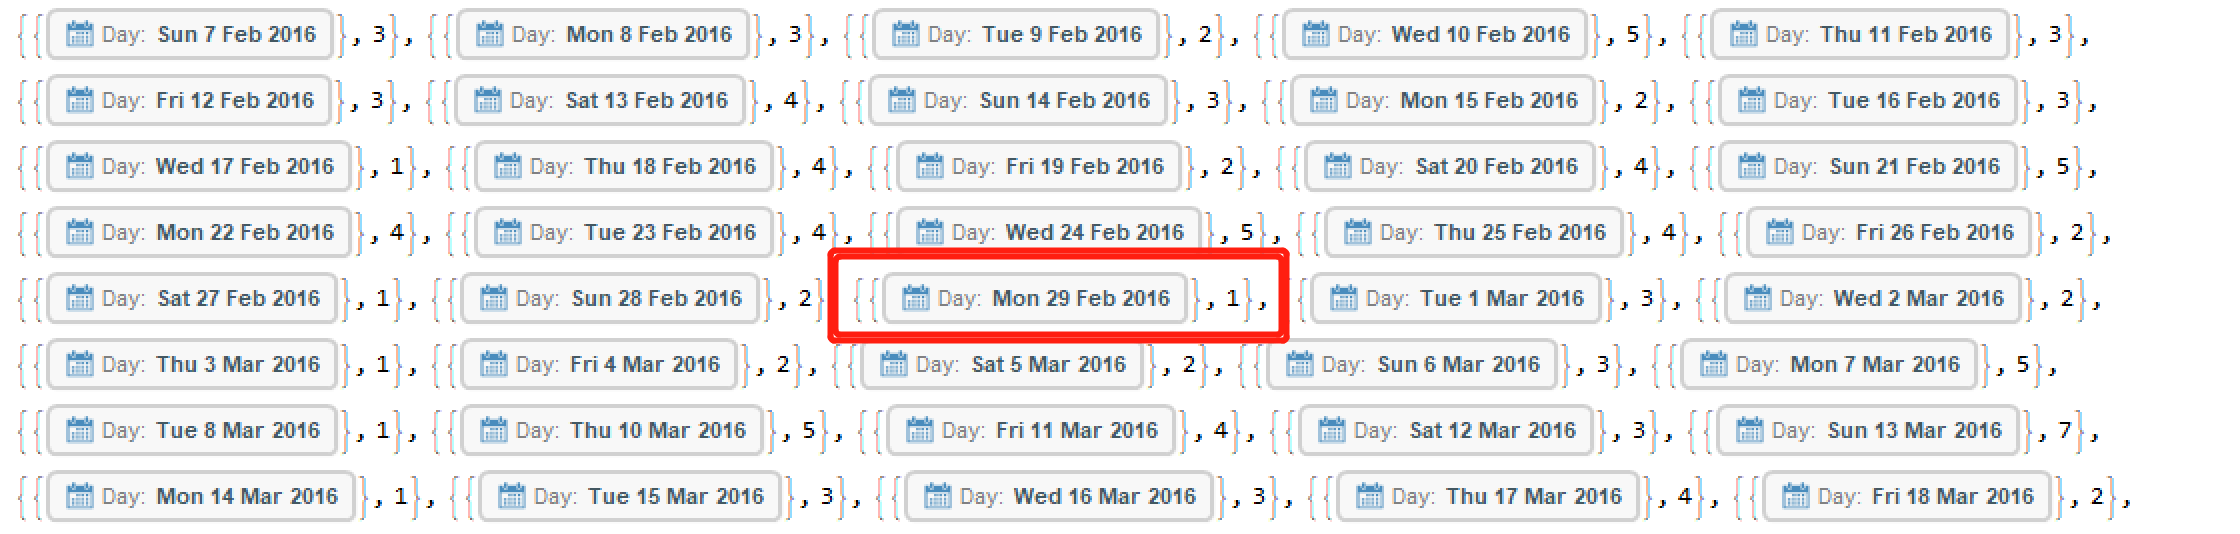
\includegraphics[width=1.1\linewidth]{leap.png}
\caption{Feb. $29^{th}$, 2016}
\end{figure}

We specificate that this day should be kept.

First, the following discussions are generally based on a unit scale of days. Removing the leap day may cause inaccurate estimation results.

Secondly, \texttt{Mathematica} supports the leap day with the plotting system. It will be extra unnecessary work to remove that from the sample.
\section{Goodness-of-Fit Test for Poisson Distribution Model}
\subsection{Objectives}
This section is oriented to question iii).

In this section, we will test whether the occurrence of police shootings in US within 2015 to 2018 follows a Poisson distribution. We set the hypothesis:
$$H_0: \text{The occurrence of police shootings in US follows a Poisson distribution with parameter }k$$
and wish not to reject it.
\subsection{Definitions and Notations}
\paragraph{Pearson's Chi-squared Goodness-of-Fit Test [2]}
Let $(X_1,\cdots,X_k)$ be a sample of size $n$ from a categorical random variable with parameters $(p_1,\cdots,p_k)$ satisfying Pearson Criteria. Let $(p_{1_0},\cdots,p_{k_0})$ be a vector of null values. Then the test
$$H0: p_i = p_{i_0},\qquad i = 1,\cdots,k$$
based on
$$\chi_{k-1}^2 = \sum^k_{i=1}\frac{(X_i-np_{i_0})^2}{np_{i_0}}$$
is called an chi-squared goodness-of-fit test.

This method allows us to test if the data conforms to an arbitrary discrete or continuous distribution, particularly,  Poisson distribution.
\paragraph{Pearson Criteria [2]}
Large $n$ is required for the chi-squared distribution to be a good approximation to the true distribution of the Pearson statistic. The general criteria is:
\begin{itemize}
\item $E[X_i] = np_i \geq 1$ for all $i = 1,\cdots,k$; 
\item $E[X_i] = np_i \geq 5$ for $80\%$ of all $i = 1,\cdots,k$.
\end{itemize}
\subsection{Goodness-of-Fit Test for 2015-2018}
To test the hypothesis, we first need to process the raw data from the \textit{Database of Fatal Police Shootings} of the Washington Post. First, we screen out the data from 2015 to 2018. Then, we use \texttt{Mathematica} to count how many times of police shooting occurs a day, and set them into different categories.

The fulfilling codes with results are:
\begin{figure}[!htbp]
\centering
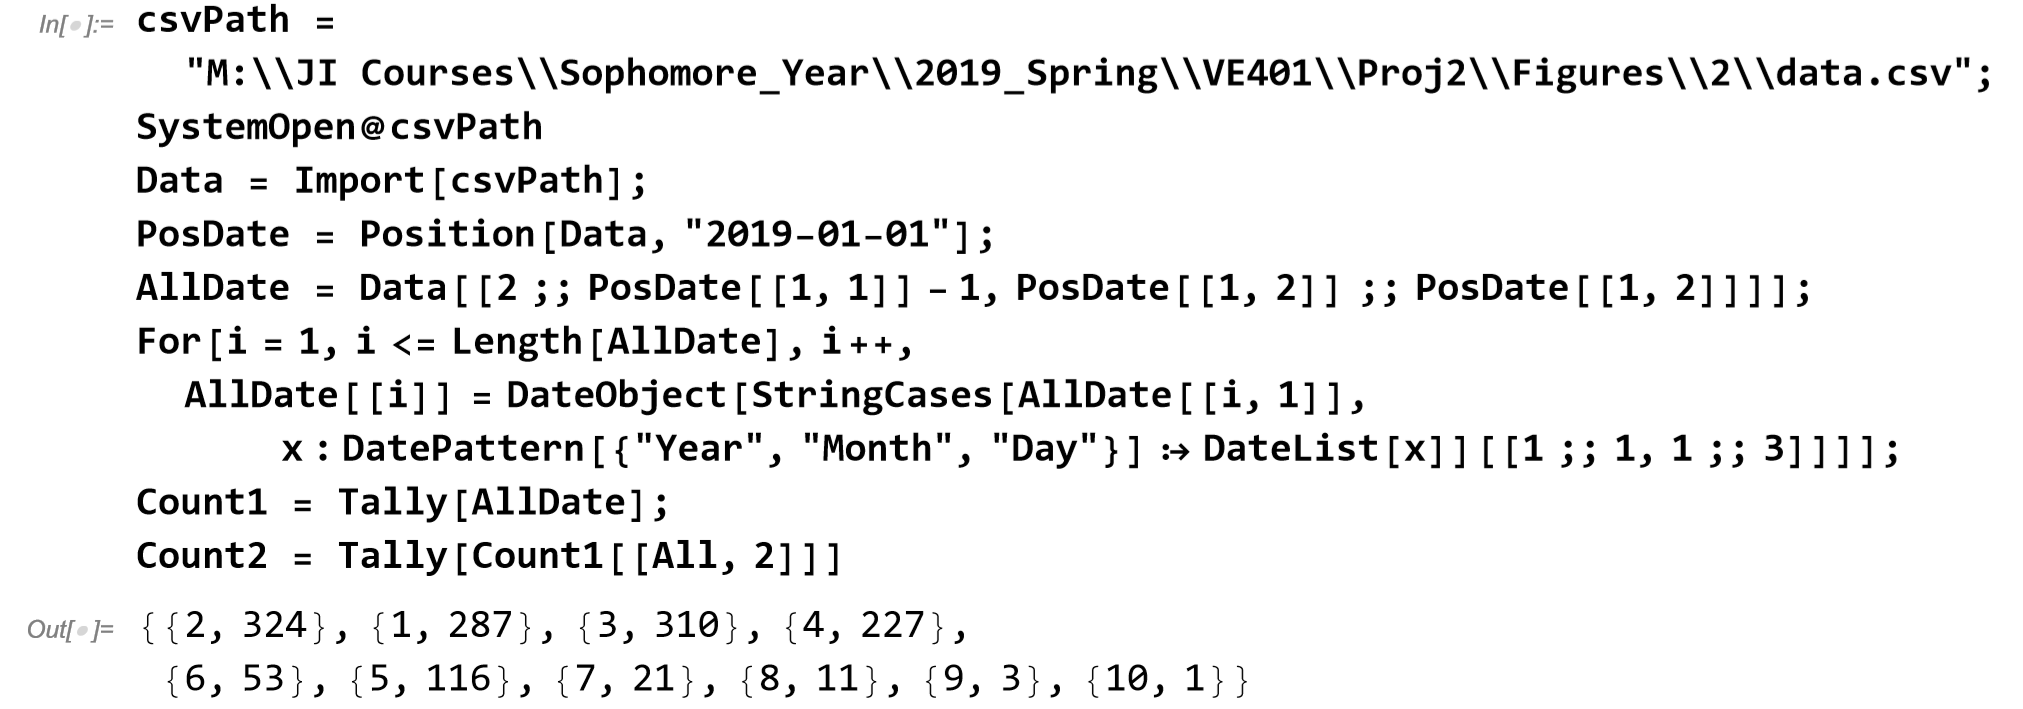
\includegraphics[width=1\linewidth]{dataprocess.png}
\end{figure}

To know the number of days of zero-shooting, we just need to use the total days minus obtained days. Note that there are 366 days in 2016!
\begin{figure}[!htbp]
\centering
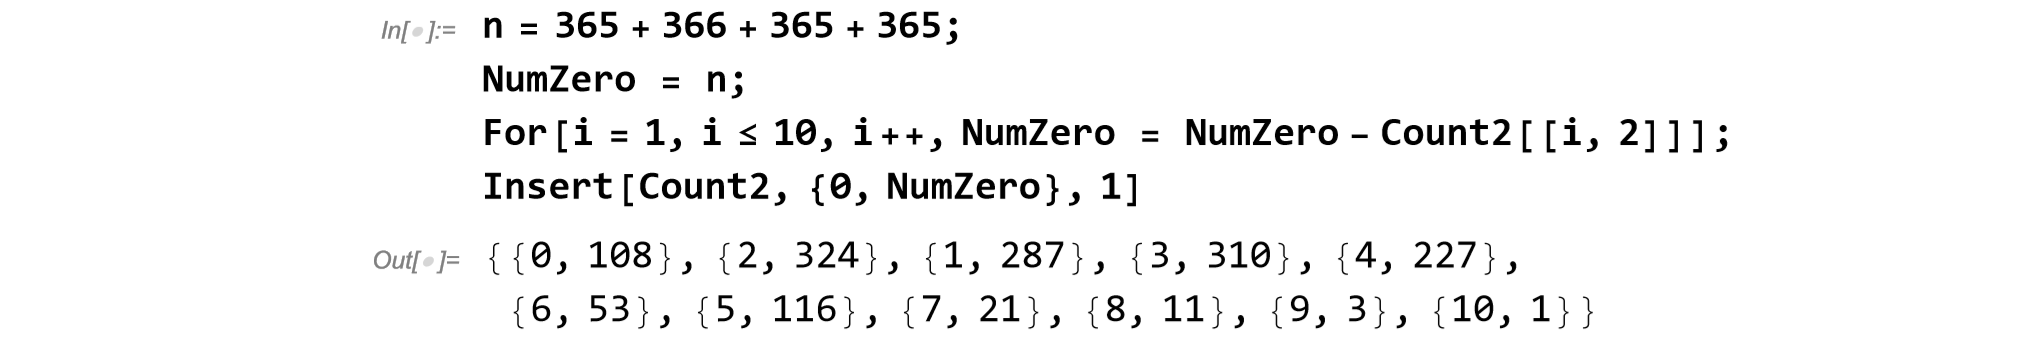
\includegraphics[width=1\linewidth]{dataprocess2.png}
\end{figure}

Reading from above coding results, we finally obtained the following data table recording occurrence of each numbers of fatal police shooting in a day.

\newpage

\begin{table}[!htbp]
\centering
\begin{tabular}{|c|c|c|c|c|c|c|c|c|c|c|c|}
\hline
Number of shooting & 0   & 1   & 2   & 3   & 4   & 5   & 6  & 7  & 8  & 9 & 10 \\ \hline
Occurrence of such day       & 108 & 287 & 324 & 310 & 227 & 116 & 53 & 21 & 11 & 3 & 1  \\ \hline
\end{tabular}
\caption{Occurrence per day table}
\end{table}

\subsubsection{Ignoring Pearson Criteria}
There is an automatic goodness-of-fit test in \texttt{Mathematica}, which ignores the Pearson Criteria. For a rough result, we plug our data table in, and the results turned out to be:

\begin{figure}[!htbp]
\centering
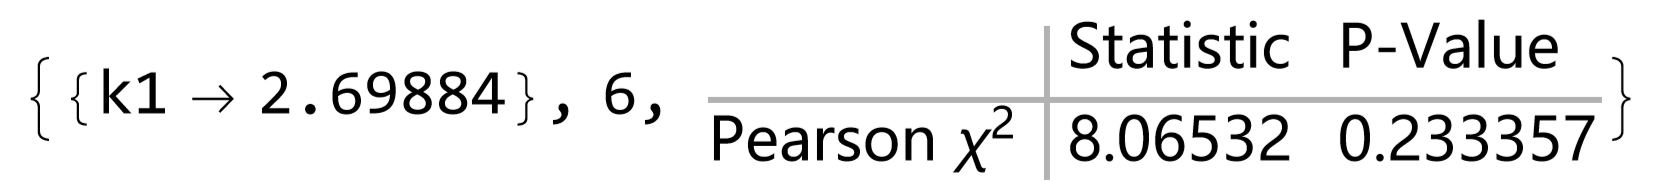
\includegraphics[width=0.6\linewidth]{poissonfit.png}
\end{figure}

Hence, we can read off that $\widehat{k}_{2019}=2.69884$. The null hypothesis is given by:
$$H_0:\text{ the number of fatal police shooting follows a Poisson distribution with parameter }\widehat{k}_{2019}=2.70$$

The $P$-value is $p=0.233$, which is large. Hence, there is no reason to believe that the number of fatal police shooting is not Poisson distributed.

\subsubsection{Considering Pearson Criteria}
To get the Pearson Statistic, we have to first find an estimator of $k$, and then calculate out the observed frequency and the expected frequency of number of police shooting occurrence per day. The expected frequency is calculated with expected probability and the total number, while the expected probability can be calculated with the formula of Poisson distribution
\begin{equation}
f(x)= \frac{e^{-\widehat{k}} \widehat{k}^x}{x!}.
\end{equation}

\paragraph{Step 1} Find an estimator for $k$.

The maximum-likelihood estimator for $\widehat{k}$ is given by the sample mean. Therefore, we can use the table above to calculate
\begin{align*}
\widehat{k}
&=\overline{X}\\
&=\displaystyle\frac{1}{365\times 4+1}(0 \times 108 + 1 \times 287 + 2 \times 324 + 3 \times 310 + 4 \times 227\\
&+ 5 \times 116 + 6 \times 53 + 7 \times 21 + 8 \times 11 + 9 \times 3 + 10 \times 1)\\
&= 2.6988
\end{align*}

\paragraph{Step 2} To apply the multinomial distribution, we calculate each element:
\begin{align*}
P[X=0] &=\displaystyle\frac{e^{-\widehat{k}}\widehat{k}^0}{0!}=0.0673\\
P[X=1] &=\displaystyle\frac{e^{-\widehat{k}}\widehat{k}^1}{1!}=0.1816\\
P[X=2] &=\displaystyle\frac{e^{-\widehat{k}}\widehat{k}^2}{2!}=0.2450\\
&\cdots \qquad \cdots\\
P[X=10] &=1-P[X=1]-\cdots-P[X=9]=0.0005
\end{align*}

The results are shown as:
\begin{table}[!htbp]
  \centering
    \begin{tabular}{cccccccccccc}
    \hline
    Num. of shoots & 0     & 1     & 2     & 3     & 4     & 5     & 6     & 7     & 8     & 9     & 10 \\
    \hline
    Category Prob. & 0.0673  & 0.1816  & 0.2450  & 0.2204  & 0.1487  & 0.0803  & 0.0361  & 0.0139  & 0.0047  & 0.0014  & 0.0005  \\
    \hline
    \end{tabular}%
    \caption{The Category Probabilities}
\end{table}%

Consider the number of shoots as categories, the Category Random Variable is given by $(0.0673,0.1816,0.2450,\\0.2204,0.1487,0.0803,0.0361,0.0139,0.0047,0.0014,0.0005)$. 

\paragraph{Step 3} Upon this, we can calculate the expected frequencies by 
$$E_i=np_i=(365\times 4+1)p_i=1461p_i.$$

For example, $E_1=1461\times 0.0673=98.302$.

All results are given by
\begin{table}[htbp]
  \centering
    \begin{tabular}{cccccccccccc}
    \hline
    Categories & 0     & 1     & 2     & 3     & 4     & 5     & 6     & 7     & 8     & 9     & 10 \\
    \hline
    Expected Freq. & 98.302  & 265.300  & 358.001  & 322.061  & 217.297  & 117.290  & 52.758  & 20.341  & 6.862  & 2.058  & 0.730  \\
    \hline
    \end{tabular}%
    \caption{The Expected Frequencies}
\end{table}%

\paragraph{Step 4} We noticed that the Pearson Criteria are not satisfied, because $E_{9-10}<5$ and $E_{10}<1$. We solve this problem by merging the last 2 categories to obtain:

\begin{table}[!htbp]
  \centering
    \begin{tabular}{ccccccccccc}
    \hline
    Categories & 0     & 1     & 2     & 3     & 4     & 5     & 6     & 7     & 8     & 9 \\
    \hline
    Expected Freq. & 98.302  & 265.300  & 358.001  & 322.061  & 217.297  & 117.290  & 52.758  & 20.341  & 6.862  & 2.788  \\
    \hline
    Observed Freq. & 108   & 287   & 324   & 310   & 227   & 116   & 53    & 21    & 11    & 4 \\
    \hline
    \end{tabular}%
    \caption{The Merged Expected and Observed Frequencies}
\end{table}%

\paragraph{Step 5}
Then we can calculate the Pearson statistic:
$$\chi_{N-1-m}^2 = \sum^k_{i=1}\frac{(X_i-np_{i_0})^2}{np_{i_0}}=\sum^k_{i=1}\frac{(O_i-E_i)^2}{E_i}$$

The degrees of freedom is found by 
$$N-1-m=10-1-1=8,$$
and the statistic is found as
\begin{figure}[!htbp]
\centering
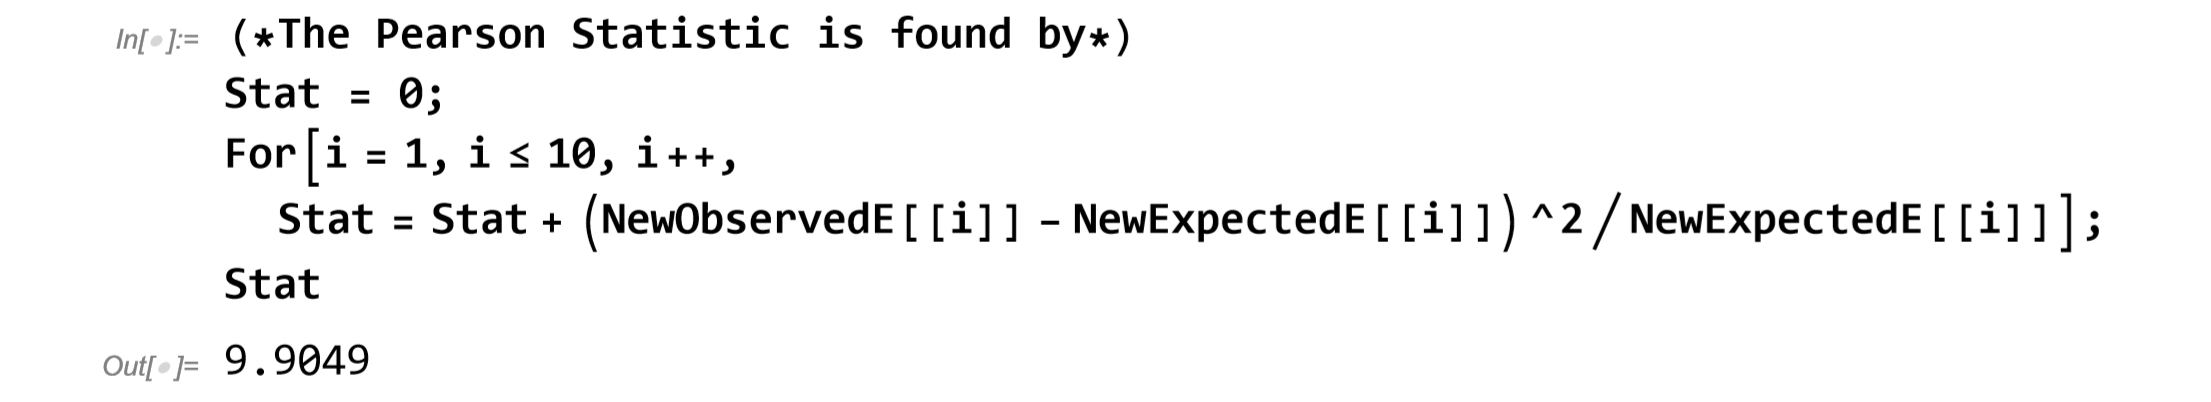
\includegraphics[width=1\linewidth]{dataprocess3.png}
\end{figure}
$$\chi_{8}^2 = 9.9049$$

\paragraph{Step 6} Fix $\alpha=0.05$, we test the null hypothesis with the $\chi^2_{0.05,8}=15.5073$. We found that
$$\chi_{8}^2 = 9.9049<15.5073=\chi^2_{0.05,8}$$

Hence we are unable to reject $H_0$.

\paragraph{Step 7} At last, we calculate the $P$-value of this test.
\begin{align*}
p &= P[\chi_{8}^2\ |\ H_0]\\
&\leq P[\chi^2\geq 9.9049] \\
&= 1-P[\chi^2\geq 9.9049]\\
&= 0.271764
\end{align*}

The $P$-value is extremely large at $27\%$ level of significance, thus we fail to reject $H_0$.

\paragraph{Conclusions}
The above calculations and tests proved that 
\begin{itemize}
\item There is no evidence to believe that Poisson distribution fails describe the number of fatal police shooting in a day. Basically, Poisson distribution gives a good approximation.
\item The Poisson parameter $k=2.6988$ in US fatal police shooting is larger than that of London Homicide $k=0.44$.
\end{itemize}
\subsection{Bar Charts of Observed and Predicted Shooting Numbers}
The barcharts are plotted by \texttt{Mathematica} (See next page).
\newpage
The observed numbers of fatal police shooting:
\begin{figure}[!htbp]
\centering
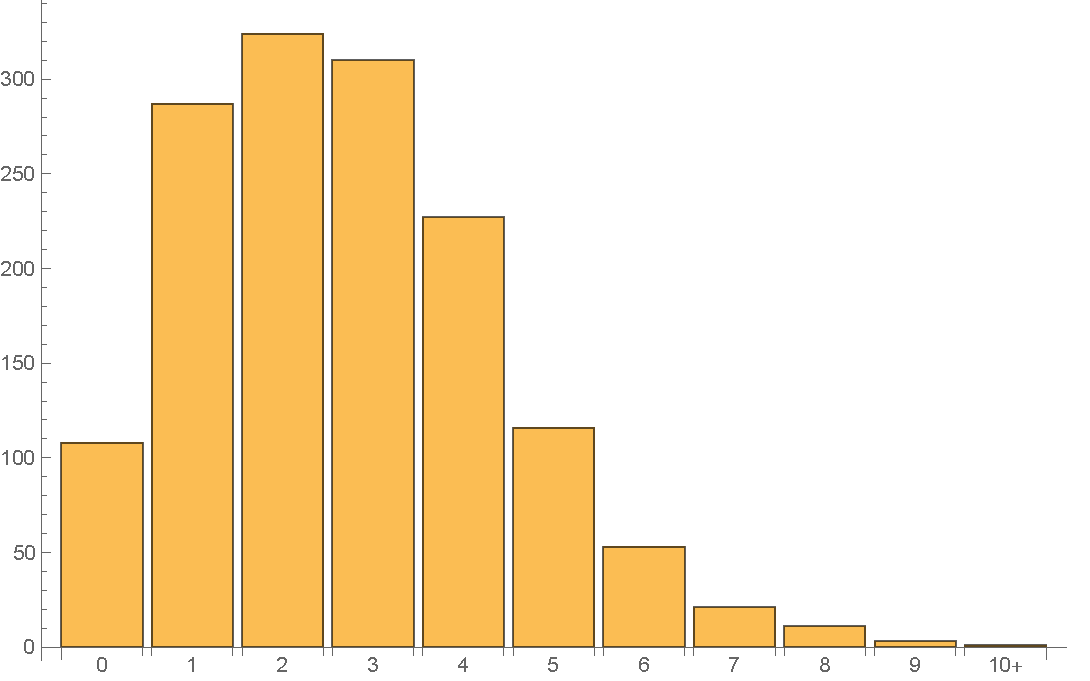
\includegraphics[width=0.8\linewidth]{observedbar.pdf}
\caption{Observed Numbers of Fatal Police Shooting}
\end{figure}

The expected numbers of fatal police shooting:
\begin{figure}[!htbp]
\centering
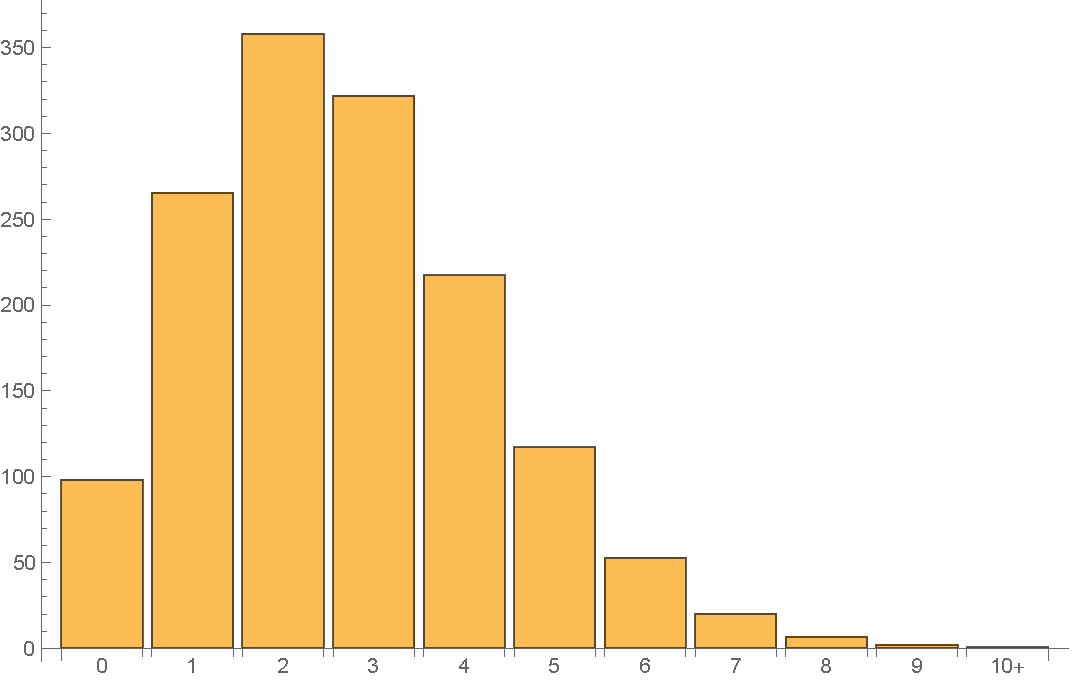
\includegraphics[width=0.8\linewidth]{expectedbar.pdf}
\caption{Expected Numbers of Fatal Police Shooting}
\end{figure}

\newpage

\section{Dependence of Average Number of Police Shooting on Weekdays}
This section is oriented to question iv).
\subsection{Objectives}
In this section, we test whether the occurrence of police shootings depends on the weekday. We first test if the average numbers follow a uniform distribution by goodness-of-fit, and then test the dependence of number of shoot and weekdays.
\subsection{Raw Data Processing}
To test whether the occurrence of police shooting depends on weekday, we first need to process the raw data from the \emph{Database of Fatal Police Shootings} of the Washington Post. We use Mathematica to count how many times of police shooting occurs for each weekday, and set them into different categories.

\begin{figure}[!htbp]
\centering
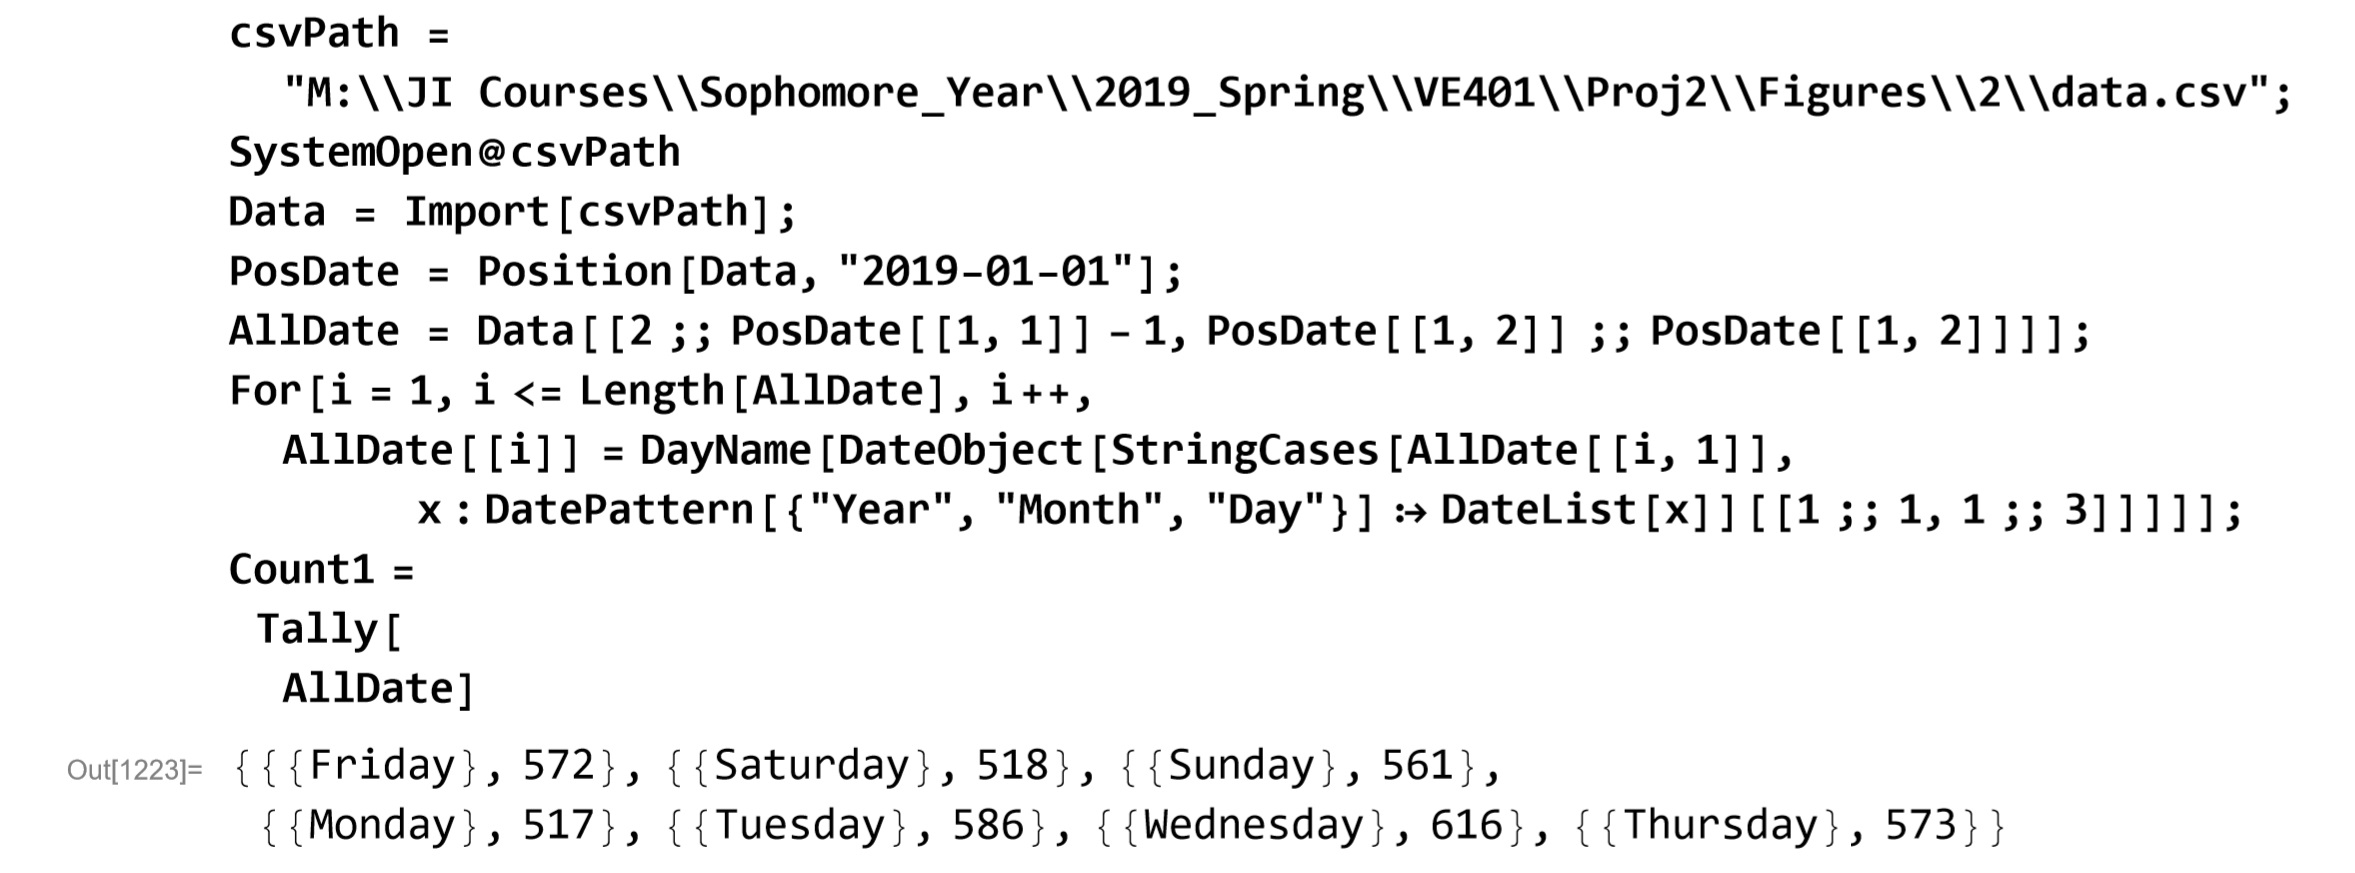
\includegraphics[width=1\linewidth]{dataprocess4.jpg}
\end{figure}

We get the total number of police-shooting occurrence for each weekday. They are 517, 586, 616, 573, 572, 518 and 561 from Monday to Sunday respectively. To make it clearer, we set a table.

\begin{table}[!htbp]
\centering
\begin{tabular}{c|ccccccc}
Day        & Monday & Tuesday & Wednesday & Thursday & Friday & Saturday & Sunday \\ \hline
Number of Occurrence & 517    & 586     & 616       & 573      & 572    & 518      & 561    \\
\end{tabular}
\caption{Number of Occurrence for Different Weekdays}
\end{table}

Upon the data, we create a histogram similar to Figure 3 of \textit{London murders: a predictable pattern?} based on data above with Mathematica.

\newpage

\begin{figure}[!htbp]
\centering
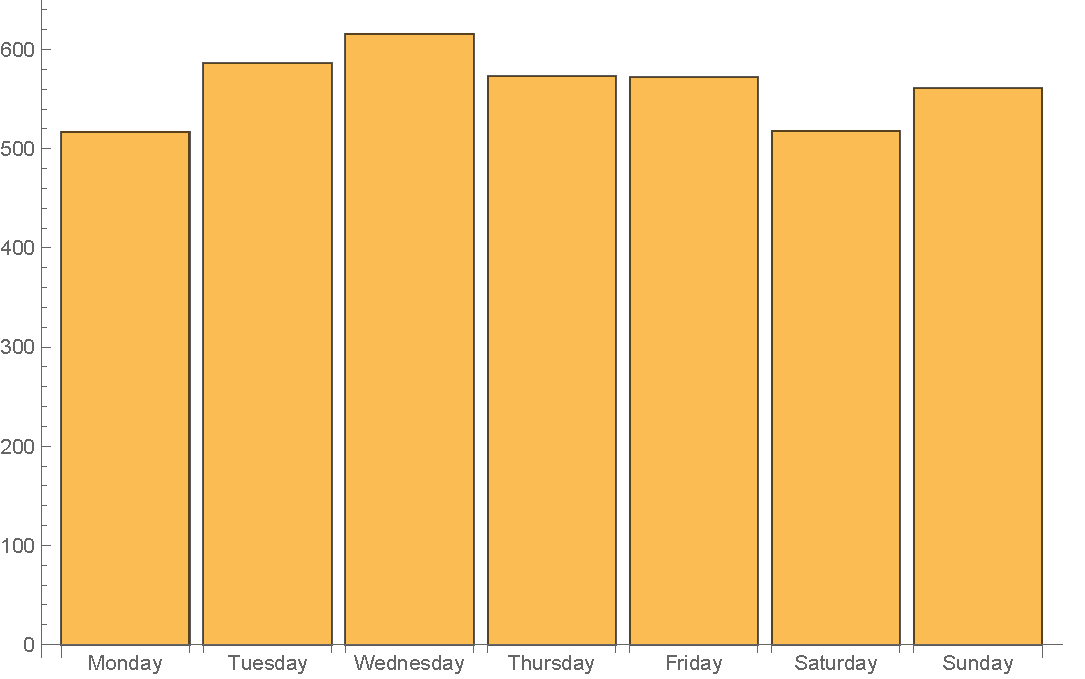
\includegraphics[width=0.8\linewidth]{occur.pdf}
\caption{Number of Occurrence for Different Weekdays}
\end{figure}

The distribution seems almost even, but is it really the case? The following tries to verify it.
\subsection{Goodness-of-fit for the Average Number of Police Shootings Depends on The Weekday}
Actually, we can interpret our testing object into another form, which is whether the occurrence of police shooting is randomly distributed among weekdays. Therefore, we want to test whether the data are uniformly distributed.

We first set our null hypothesis
\begin{equation*}
H_0: \text{The data follow a multinomial distribution with parameters} \left( p _ { 1 } , \ldots , p _ { 7 } \right) = \left( \frac { 1 } { 7 } , \ldots , \frac { 1 } { 7 } \right)
\end{equation*}

\paragraph{Step 1} We calculate the average occurrence of each weekday, by processing the data above:
$$\text{Average Shoot} = \frac{\text{Total Shoot}}{\text{Number of Days}}$$

In the time period, there is a total of 208 Tuesdays and Wednesdays, and 209 for the rest. By code, we find out the average:

\newpage

\begin{figure}[!htbp]
\centering
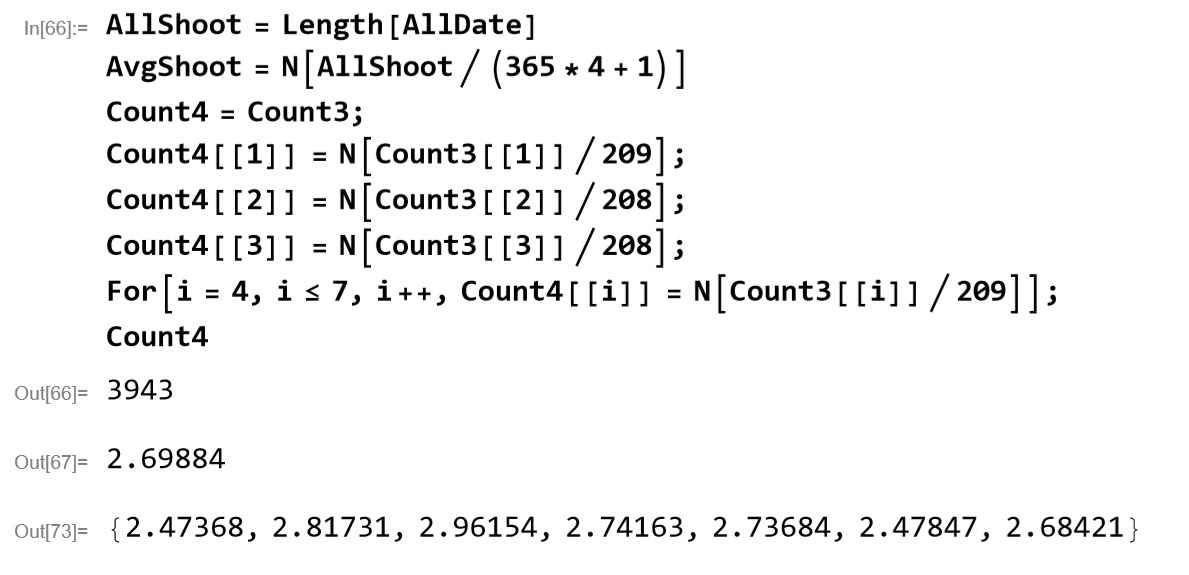
\includegraphics[width=0.8\linewidth]{dataprocess5.jpg}
\end{figure}

Hence we received the observed data as the following table.

\begin{table}[!htbp]
\centering
\begin{tabular}{c|ccccccc|c}
                    & Monday  & Tuesday & Wednesday & Thursday & Friday  & Saturday & Sunday  & Total \\ \hline
Observed Occurrence & 2.474     & 2.817     & 2.962       & 2.742      & 2.737     & 2.478      & 2.684     & 18.894  \\ 
\end{tabular}
\caption{Average Observed Occurrence}
\end{table}

\paragraph{Step 2} We then find the expected occurrence. This can be found by
$$E_i = np_i$$

For uniform distribution, all $E_i$s are given by
$$E=np=\frac{3943}{1461}=2.699$$

Thus we gain a table of expected average occurrence of police shooting for different weekdays.

\begin{table}[!htbp]
\centering
\begin{tabular}{c|ccccccc|c}
                    & Monday  & Tuesday & Wednesday & Thursday & Friday  & Saturday & Sunday  & Total \\ \hline
Observed Occurrence & 2.474     & 2.817     & 2.962       & 2.742      & 2.737     & 2.478      & 2.684     & 18.894  \\ \hline
Expected Occurrence & 2.699 & 2.699 & 2.699   & 2.699  & 2.699 & 2.699  & 2.699 & 18.892  \\
\end{tabular}
\caption{Average Observed and Expected Occurrence}
\end{table}

\paragraph{Step 3} We then find the Pearson statistic.

It follows a chi-squared distribution with $$7-1=6$$ degrees of freedom.

The observed test statistic is
\begin{equation}
\sum _ { i = 1 } ^ { 7 } \frac { \left( O _ { i } - E _ { i } \right) ^{ 2 } } { E _ { i } } = \frac { ( 2.474 – 2.699 ) ^ { 2 } } { 2.699 } + \cdots + \frac { ( 2.684 – 2.699 ) ^ { 2 } } { 2.699 } = 0.069
\end{equation}

\paragraph{Step 4}Fix $\alpha=0.05$, we test the null hypothesis with the $\chi^2_{0.05,6}=12.592$. We found that
$$\chi_{6}^2 = 0.069<12.592=\chi^2_{0.05,6}$$

0.069 is much less than 12.592. Hence we are unable to reject $H_0$.

\paragraph{Step 5} At last, we calculate the $P$-value of this test.
\begin{align*}
p &= P[\chi_{6}^2\ |\ H_0]\\
&\leq P[\chi^2\geq 0.069] \\
&= 1-P[\chi^2\geq 0.069]\\
&= 0.999993
\end{align*}

The $P$-value is extremely large at more than $99\%$ level of significance, thus we fail to reject $H_0$.

Therefore, there is no evidence that the average occurrence of police shooting is not randomly distributed. 

We draw our final conclusion that there is no evidence that the average number of police shootings depends on the weekday.

\subsection{Independence Test for Number of Shoot and Weekdays}
But is the number of shoots really independent of weekdays? To find out, we perform independence test. We set $H_0$ that there is no dependence.

\paragraph{Step 1} We first process the rough data by \texttt{Mathematica}. We want the numbers of the day with certain number of shoots. The results are:

\begin{figure}[!htbp]
\centering
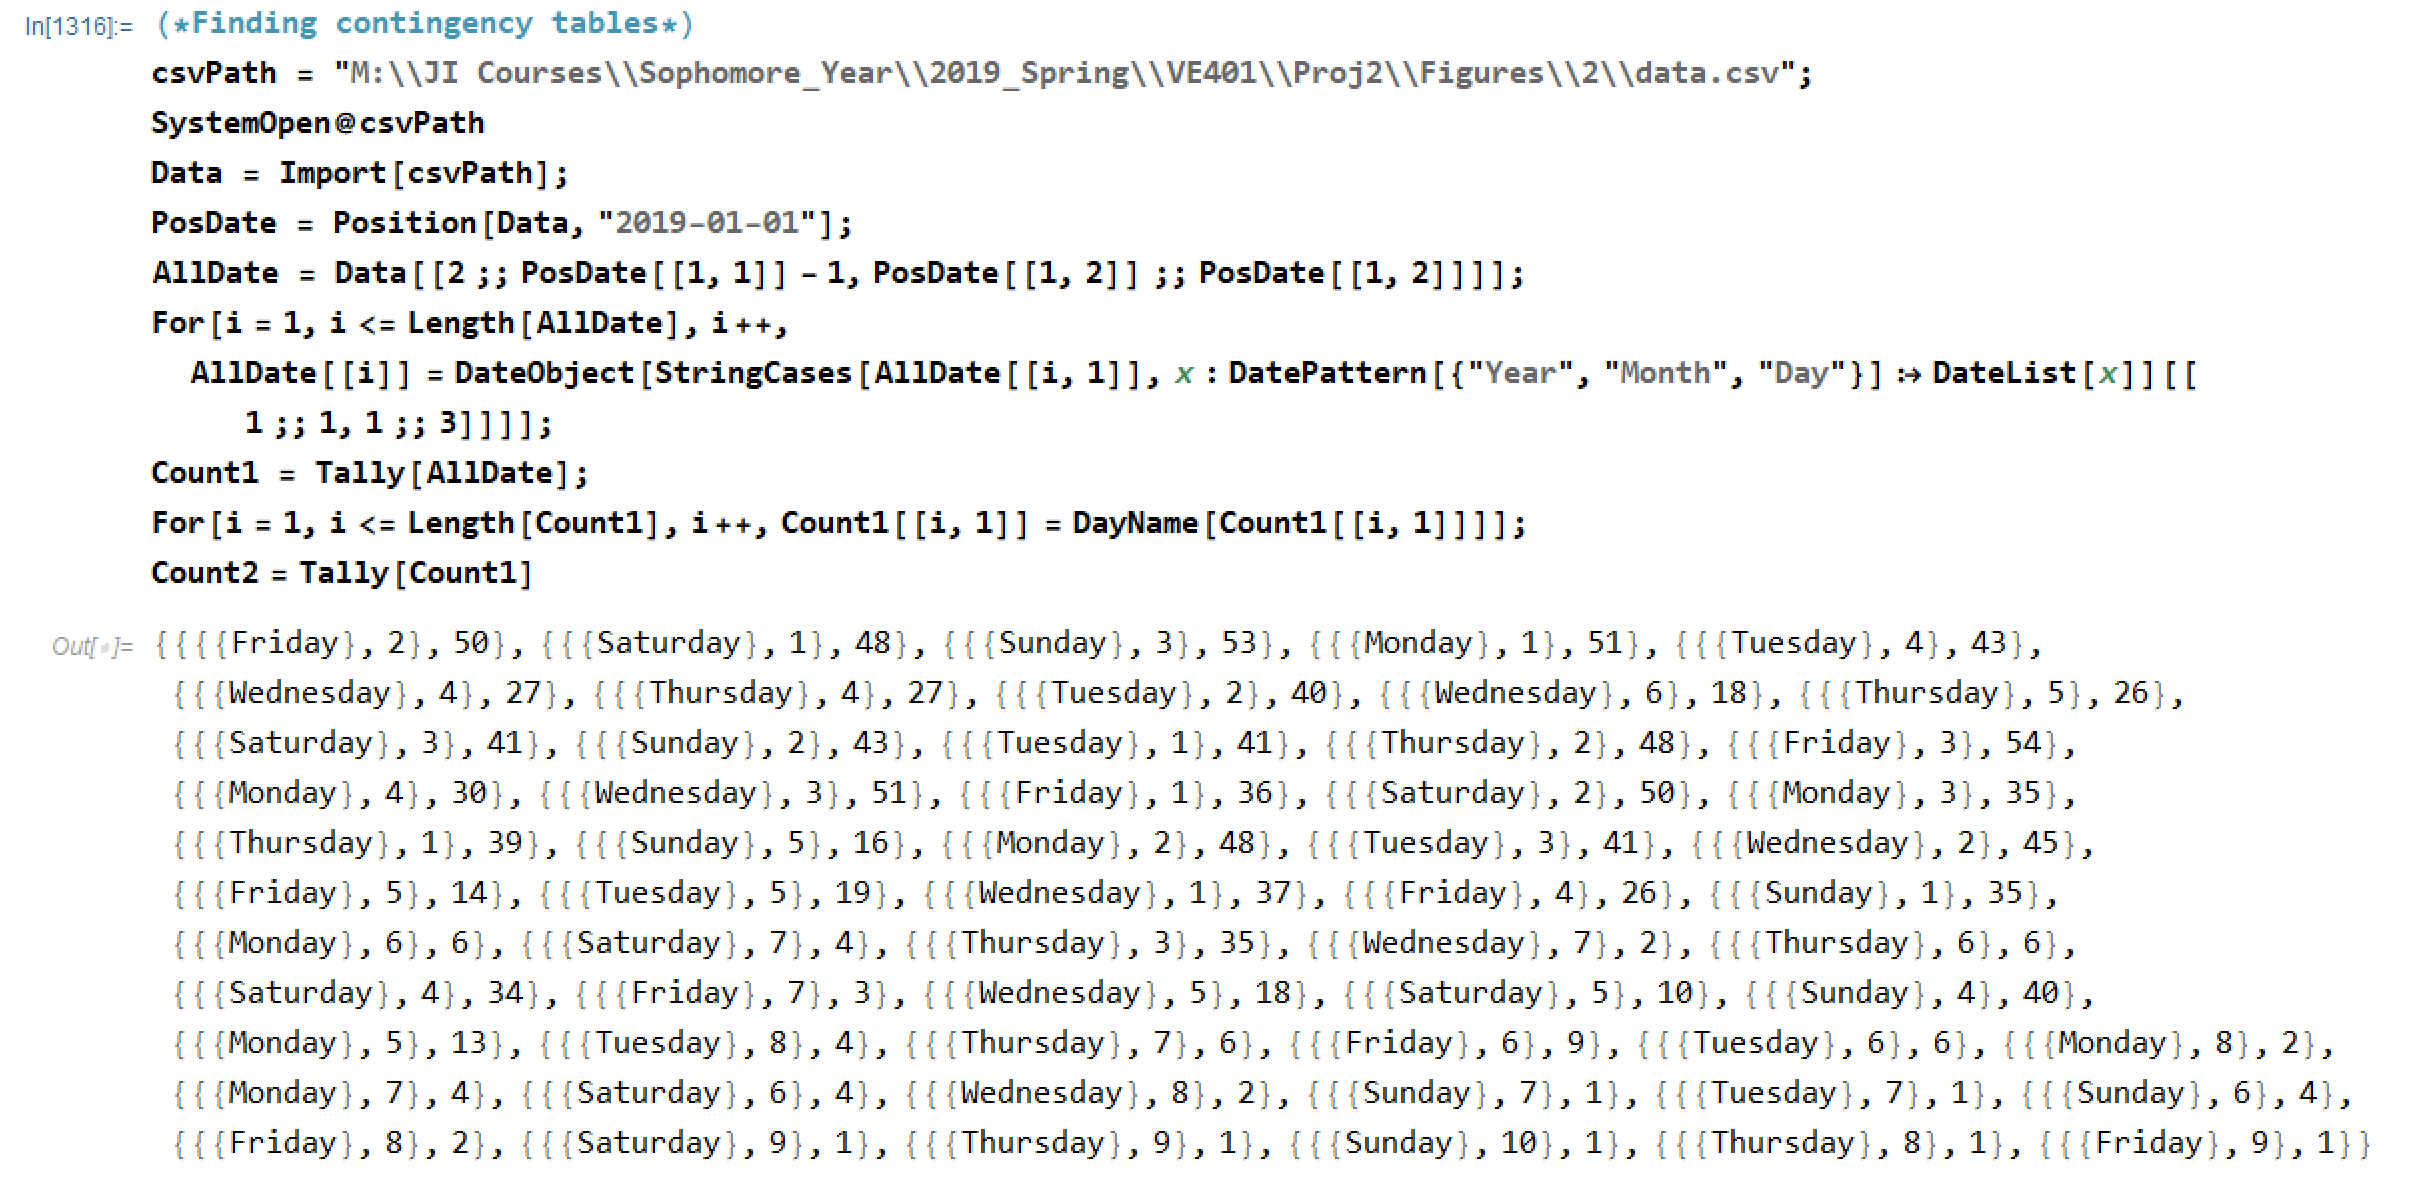
\includegraphics[width=1.1\linewidth]{dataprocess6.png}
\end{figure}

\newpage

The results are summarized in the contingency table.

\begin{table}[!htbp]
  \centering
    \begin{tabular}{|c|c|c|c|c|c|c|c|c|c|c|c|c|}
    \hline
    \rowcolor[rgb]{ .867,  .922,  .969} Numbers of shoots & 0     & 1     & 2     & 3     & 4     & 5     & 6     & 7     & 8     & 9     & 10    & Total \\
    \hline
    \rowcolor[rgb]{ .867,  .922,  .969} Monday & \cellcolor[rgb]{ 1,  1,  1}20 & \cellcolor[rgb]{ 1,  1,  1}51 & \cellcolor[rgb]{ 1,  1,  1}48 & \cellcolor[rgb]{ 1,  1,  1}35 & \cellcolor[rgb]{ 1,  1,  1}30 & \cellcolor[rgb]{ 1,  1,  1}13 & \cellcolor[rgb]{ 1,  1,  1}6 & \cellcolor[rgb]{ 1,  1,  1}4 & \cellcolor[rgb]{ 1,  1,  1}2 & \cellcolor[rgb]{ 1,  1,  1}0 & \cellcolor[rgb]{ 1,  1,  1}0 & 209 \\
    \hline
    \rowcolor[rgb]{ .867,  .922,  .969} Tuesday & \cellcolor[rgb]{ 1,  1,  1}13 & \cellcolor[rgb]{ 1,  1,  1}41 & \cellcolor[rgb]{ 1,  1,  1}40 & \cellcolor[rgb]{ 1,  1,  1}41 & \cellcolor[rgb]{ 1,  1,  1}43 & \cellcolor[rgb]{ 1,  1,  1}19 & \cellcolor[rgb]{ 1,  1,  1}6 & \cellcolor[rgb]{ 1,  1,  1}1 & \cellcolor[rgb]{ 1,  1,  1}4 & \cellcolor[rgb]{ 1,  1,  1}0 & \cellcolor[rgb]{ 1,  1,  1}0 & 208 \\
    \hline
    \rowcolor[rgb]{ .867,  .922,  .969} Wednesday & \cellcolor[rgb]{ 1,  1,  1}8 & \cellcolor[rgb]{ 1,  1,  1}37 & \cellcolor[rgb]{ 1,  1,  1}45 & \cellcolor[rgb]{ 1,  1,  1}51 & \cellcolor[rgb]{ 1,  1,  1}27 & \cellcolor[rgb]{ 1,  1,  1}18 & \cellcolor[rgb]{ 1,  1,  1}18 & \cellcolor[rgb]{ 1,  1,  1}2 & \cellcolor[rgb]{ 1,  1,  1}2 & \cellcolor[rgb]{ 1,  1,  1}0 & \cellcolor[rgb]{ 1,  1,  1}0 & 208 \\
    \hline
    \rowcolor[rgb]{ .867,  .922,  .969} Thursday & \cellcolor[rgb]{ 1,  1,  1}20 & \cellcolor[rgb]{ 1,  1,  1}39 & \cellcolor[rgb]{ 1,  1,  1}48 & \cellcolor[rgb]{ 1,  1,  1}35 & \cellcolor[rgb]{ 1,  1,  1}27 & \cellcolor[rgb]{ 1,  1,  1}26 & \cellcolor[rgb]{ 1,  1,  1}6 & \cellcolor[rgb]{ 1,  1,  1}6 & \cellcolor[rgb]{ 1,  1,  1}1 & \cellcolor[rgb]{ 1,  1,  1}1 & \cellcolor[rgb]{ 1,  1,  1}0 & 209 \\
    \hline
    \rowcolor[rgb]{ .867,  .922,  .969} Friday & \cellcolor[rgb]{ 1,  1,  1}14 & \cellcolor[rgb]{ 1,  1,  1}36 & \cellcolor[rgb]{ 1,  1,  1}50 & \cellcolor[rgb]{ 1,  1,  1}54 & \cellcolor[rgb]{ 1,  1,  1}26 & \cellcolor[rgb]{ 1,  1,  1}14 & \cellcolor[rgb]{ 1,  1,  1}9 & \cellcolor[rgb]{ 1,  1,  1}3 & \cellcolor[rgb]{ 1,  1,  1}2 & \cellcolor[rgb]{ 1,  1,  1}1 & \cellcolor[rgb]{ 1,  1,  1}0 & 209 \\
    \hline
    \rowcolor[rgb]{ .867,  .922,  .969} Saturday & \cellcolor[rgb]{ 1,  1,  1}17 & \cellcolor[rgb]{ 1,  1,  1}48 & \cellcolor[rgb]{ 1,  1,  1}50 & \cellcolor[rgb]{ 1,  1,  1}41 & \cellcolor[rgb]{ 1,  1,  1}34 & \cellcolor[rgb]{ 1,  1,  1}10 & \cellcolor[rgb]{ 1,  1,  1}4 & \cellcolor[rgb]{ 1,  1,  1}4 & \cellcolor[rgb]{ 1,  1,  1}0 & \cellcolor[rgb]{ 1,  1,  1}1 & \cellcolor[rgb]{ 1,  1,  1}0 & 209 \\
    \hline
    \rowcolor[rgb]{ .867,  .922,  .969} Sunday & \cellcolor[rgb]{ 1,  1,  1}16 & \cellcolor[rgb]{ 1,  1,  1}35 & \cellcolor[rgb]{ 1,  1,  1}43 & \cellcolor[rgb]{ 1,  1,  1}53 & \cellcolor[rgb]{ 1,  1,  1}40 & \cellcolor[rgb]{ 1,  1,  1}16 & \cellcolor[rgb]{ 1,  1,  1}4 & \cellcolor[rgb]{ 1,  1,  1}1 & \cellcolor[rgb]{ 1,  1,  1}0 & \cellcolor[rgb]{ 1,  1,  1}0 & \cellcolor[rgb]{ 1,  1,  1}1 & 209 \\
    \hline
    \rowcolor[rgb]{ .867,  .922,  .969} Total & 108   & 287   & 324   & 310   & 227   & 116   & 53    & 21    & 11    & 3     & 1     & 1461 \\
    \hline
    \end{tabular}%
    \caption{Contingency Table}
\end{table}%

\paragraph{Step 2} Find the expected frequencies.

The expected frequencies are found by 
$$E_{ij} = n\cdot \widehat{p_{ij}}$$

Hence the table is given by:
\begin{table}[!htbp]
  \centering
    \begin{tabular}{|c|c|c|c|c|c|c|c|c|c|c|c|}
    \hline
    \rowcolor[rgb]{ .867,  .922,  .969} Numbers of shoots & 0     & 1     & 2     & 3     & 4     & 5     & 6     & 7     & 8     & 9     & 10 \\
    \hline
    \rowcolor[rgb]{ .867,  .922,  .969} Monday & \cellcolor[rgb]{ 1,  1,  1}15.45  & \cellcolor[rgb]{ 1,  1,  1}41.06  & \cellcolor[rgb]{ 1,  1,  1}46.35  & \cellcolor[rgb]{ 1,  1,  1}44.35  & \cellcolor[rgb]{ 1,  1,  1}32.47  & \cellcolor[rgb]{ 1,  1,  1}16.59  & \cellcolor[rgb]{ 1,  1,  1}7.58  & \cellcolor[rgb]{ 1,  1,  1}3.00  & \cellcolor[rgb]{ 1,  1,  1}1.57  & \cellcolor[rgb]{ 1,  1,  1}0.43  & \cellcolor[rgb]{ 1,  1,  1}0.14  \\
    \hline
    \rowcolor[rgb]{ .867,  .922,  .969} Tuesday & \cellcolor[rgb]{ 1,  1,  1}15.38  & \cellcolor[rgb]{ 1,  1,  1}40.86  & \cellcolor[rgb]{ 1,  1,  1}46.13  & \cellcolor[rgb]{ 1,  1,  1}44.13  & \cellcolor[rgb]{ 1,  1,  1}32.32  & \cellcolor[rgb]{ 1,  1,  1}16.51  & \cellcolor[rgb]{ 1,  1,  1}7.55  & \cellcolor[rgb]{ 1,  1,  1}2.99  & \cellcolor[rgb]{ 1,  1,  1}1.57  & \cellcolor[rgb]{ 1,  1,  1}0.43  & \cellcolor[rgb]{ 1,  1,  1}0.14  \\
    \hline
    \rowcolor[rgb]{ .867,  .922,  .969} Wednesday & \cellcolor[rgb]{ 1,  1,  1}15.38  & \cellcolor[rgb]{ 1,  1,  1}40.86  & \cellcolor[rgb]{ 1,  1,  1}46.13  & \cellcolor[rgb]{ 1,  1,  1}44.13  & \cellcolor[rgb]{ 1,  1,  1}32.32  & \cellcolor[rgb]{ 1,  1,  1}16.51  & \cellcolor[rgb]{ 1,  1,  1}7.55  & \cellcolor[rgb]{ 1,  1,  1}2.99  & \cellcolor[rgb]{ 1,  1,  1}1.57  & \cellcolor[rgb]{ 1,  1,  1}0.43  & \cellcolor[rgb]{ 1,  1,  1}0.14  \\
    \hline
    \rowcolor[rgb]{ .867,  .922,  .969} Thursday & \cellcolor[rgb]{ 1,  1,  1}15.45  & \cellcolor[rgb]{ 1,  1,  1}41.06  & \cellcolor[rgb]{ 1,  1,  1}46.35  & \cellcolor[rgb]{ 1,  1,  1}44.35  & \cellcolor[rgb]{ 1,  1,  1}32.47  & \cellcolor[rgb]{ 1,  1,  1}16.59  & \cellcolor[rgb]{ 1,  1,  1}7.58  & \cellcolor[rgb]{ 1,  1,  1}3.00  & \cellcolor[rgb]{ 1,  1,  1}1.57  & \cellcolor[rgb]{ 1,  1,  1}0.43  & \cellcolor[rgb]{ 1,  1,  1}0.14  \\
    \hline
    \rowcolor[rgb]{ .867,  .922,  .969} Friday & \cellcolor[rgb]{ 1,  1,  1}15.45  & \cellcolor[rgb]{ 1,  1,  1}41.06  & \cellcolor[rgb]{ 1,  1,  1}46.35  & \cellcolor[rgb]{ 1,  1,  1}44.35  & \cellcolor[rgb]{ 1,  1,  1}32.47  & \cellcolor[rgb]{ 1,  1,  1}16.59  & \cellcolor[rgb]{ 1,  1,  1}7.58  & \cellcolor[rgb]{ 1,  1,  1}3.00  & \cellcolor[rgb]{ 1,  1,  1}1.57  & \cellcolor[rgb]{ 1,  1,  1}0.43  & \cellcolor[rgb]{ 1,  1,  1}0.14  \\
    \hline
    \rowcolor[rgb]{ .867,  .922,  .969} Saturday & \cellcolor[rgb]{ 1,  1,  1}15.45  & \cellcolor[rgb]{ 1,  1,  1}41.06  & \cellcolor[rgb]{ 1,  1,  1}46.35  & \cellcolor[rgb]{ 1,  1,  1}44.35  & \cellcolor[rgb]{ 1,  1,  1}32.47  & \cellcolor[rgb]{ 1,  1,  1}16.59  & \cellcolor[rgb]{ 1,  1,  1}7.58  & \cellcolor[rgb]{ 1,  1,  1}3.00  & \cellcolor[rgb]{ 1,  1,  1}1.57  & \cellcolor[rgb]{ 1,  1,  1}0.43  & \cellcolor[rgb]{ 1,  1,  1}0.14  \\
    \hline
    \rowcolor[rgb]{ .867,  .922,  .969} Sunday & \cellcolor[rgb]{ 1,  1,  1}15.45  & \cellcolor[rgb]{ 1,  1,  1}41.06  & \cellcolor[rgb]{ 1,  1,  1}46.35  & \cellcolor[rgb]{ 1,  1,  1}44.35  & \cellcolor[rgb]{ 1,  1,  1}32.47  & \cellcolor[rgb]{ 1,  1,  1}16.59  & \cellcolor[rgb]{ 1,  1,  1}7.58  & \cellcolor[rgb]{ 1,  1,  1}3.00  & \cellcolor[rgb]{ 1,  1,  1}1.57  & \cellcolor[rgb]{ 1,  1,  1}0.43  & \cellcolor[rgb]{ 1,  1,  1}0.14  \\
    \hline
    \end{tabular}%
  \caption{Expected Frequencies}
\end{table}%

\paragraph{Step 3} Then we find the Pearson statistics.
$$\chi^2 = \sum \frac { \left( O _ { i } - E _ { i } \right) ^{ 2 } } { E _ { i } }$$

The individual adders are presented by:

\newpage

\begin{table}[!htbp]
  \centering
    \begin{tabular}{|c|c|c|c|c|c|c|c|c|c|c|c|}
    \hline
    \rowcolor[rgb]{ .867,  .922,  .969} Numbers of shoots & 0     & 1     & 2     & 3     & 4     & 5     & 6     & 7     & 8     & 9     & 10 \\
    \hline
    \rowcolor[rgb]{ .867,  .922,  .969} Monday & \cellcolor[rgb]{ 1,  1,  1}1.34  & \cellcolor[rgb]{ 1,  1,  1}2.41  & \cellcolor[rgb]{ 1,  1,  1}0.06  & \cellcolor[rgb]{ 1,  1,  1}1.97  & \cellcolor[rgb]{ 1,  1,  1}0.19  & \cellcolor[rgb]{ 1,  1,  1}0.78  & \cellcolor[rgb]{ 1,  1,  1}0.33  & \cellcolor[rgb]{ 1,  1,  1}0.33  & \cellcolor[rgb]{ 1,  1,  1}0.12  & \cellcolor[rgb]{ 1,  1,  1}0.43  & \cellcolor[rgb]{ 1,  1,  1}0.14  \\
    \hline
    \rowcolor[rgb]{ .867,  .922,  .969} Tuesday & \cellcolor[rgb]{ 1,  1,  1}0.37  & \cellcolor[rgb]{ 1,  1,  1}0.00  & \cellcolor[rgb]{ 1,  1,  1}0.81  & \cellcolor[rgb]{ 1,  1,  1}0.22  & \cellcolor[rgb]{ 1,  1,  1}3.53  & \cellcolor[rgb]{ 1,  1,  1}0.37  & \cellcolor[rgb]{ 1,  1,  1}0.32  & \cellcolor[rgb]{ 1,  1,  1}1.32  & \cellcolor[rgb]{ 1,  1,  1}3.78  & \cellcolor[rgb]{ 1,  1,  1}0.43  & \cellcolor[rgb]{ 1,  1,  1}0.14  \\
    \hline
    \rowcolor[rgb]{ .867,  .922,  .969} Wednesday & \cellcolor[rgb]{ 1,  1,  1}3.54  & \cellcolor[rgb]{ 1,  1,  1}0.36  & \cellcolor[rgb]{ 1,  1,  1}0.03  & \cellcolor[rgb]{ 1,  1,  1}1.07  & \cellcolor[rgb]{ 1,  1,  1}0.87  & \cellcolor[rgb]{ 1,  1,  1}0.13  & \cellcolor[rgb]{ 1,  1,  1}14.48  & \cellcolor[rgb]{ 1,  1,  1}0.33  & \cellcolor[rgb]{ 1,  1,  1}0.12  & \cellcolor[rgb]{ 1,  1,  1}0.43  & \cellcolor[rgb]{ 1,  1,  1}0.14  \\
    \hline
    \rowcolor[rgb]{ .867,  .922,  .969} Thursday & \cellcolor[rgb]{ 1,  1,  1}1.34  & \cellcolor[rgb]{ 1,  1,  1}0.10  & \cellcolor[rgb]{ 1,  1,  1}0.06  & \cellcolor[rgb]{ 1,  1,  1}1.97  & \cellcolor[rgb]{ 1,  1,  1}0.92  & \cellcolor[rgb]{ 1,  1,  1}5.33  & \cellcolor[rgb]{ 1,  1,  1}0.33  & \cellcolor[rgb]{ 1,  1,  1}2.99  & \cellcolor[rgb]{ 1,  1,  1}0.21  & \cellcolor[rgb]{ 1,  1,  1}0.76  & \cellcolor[rgb]{ 1,  1,  1}0.14  \\
    \hline
    \rowcolor[rgb]{ .867,  .922,  .969} Friday & \cellcolor[rgb]{ 1,  1,  1}0.14  & \cellcolor[rgb]{ 1,  1,  1}0.62  & \cellcolor[rgb]{ 1,  1,  1}0.29  & \cellcolor[rgb]{ 1,  1,  1}2.10  & \cellcolor[rgb]{ 1,  1,  1}1.29  & \cellcolor[rgb]{ 1,  1,  1}0.41  & \cellcolor[rgb]{ 1,  1,  1}0.27  & \cellcolor[rgb]{ 1,  1,  1}0.00  & \cellcolor[rgb]{ 1,  1,  1}0.12  & \cellcolor[rgb]{ 1,  1,  1}0.76  & \cellcolor[rgb]{ 1,  1,  1}0.14  \\
    \hline
    \rowcolor[rgb]{ .867,  .922,  .969} Saturday & \cellcolor[rgb]{ 1,  1,  1}0.16  & \cellcolor[rgb]{ 1,  1,  1}1.17  & \cellcolor[rgb]{ 1,  1,  1}0.29  & \cellcolor[rgb]{ 1,  1,  1}0.25  & \cellcolor[rgb]{ 1,  1,  1}0.07  & \cellcolor[rgb]{ 1,  1,  1}2.62  & \cellcolor[rgb]{ 1,  1,  1}1.69  & \cellcolor[rgb]{ 1,  1,  1}0.33  & \cellcolor[rgb]{ 1,  1,  1}1.57  & \cellcolor[rgb]{ 1,  1,  1}0.76  & \cellcolor[rgb]{ 1,  1,  1}0.14  \\
    \hline
    \rowcolor[rgb]{ .867,  .922,  .969} Sunday & \cellcolor[rgb]{ 1,  1,  1}0.02  & \cellcolor[rgb]{ 1,  1,  1}0.89  & \cellcolor[rgb]{ 1,  1,  1}0.24  & \cellcolor[rgb]{ 1,  1,  1}1.69  & \cellcolor[rgb]{ 1,  1,  1}1.74  & \cellcolor[rgb]{ 1,  1,  1}0.02  & \cellcolor[rgb]{ 1,  1,  1}1.69  & \cellcolor[rgb]{ 1,  1,  1}1.34  & \cellcolor[rgb]{ 1,  1,  1}1.57  & \cellcolor[rgb]{ 1,  1,  1}0.43  & \cellcolor[rgb]{ 1,  1,  1}5.13  \\
    \hline
    \end{tabular}%
  \caption{Each Adders in Pearson Statistic}
\end{table}%

The degrees of freedom is 
$$(11-1)\times(7-1)=60$$

Hence the statistic is
$$\chi_{60}^2=\sum^{7}_{i=1} \sum^{11}_{j=1} \frac { \left( O _ { ij } - E _ { ij } \right) ^{ 2 } } { E _ { ij } } = 85.02$$

\paragraph{Step 4}Fix $\alpha=0.05$, we test the null hypothesis with the $\chi^2_{0.05,60}=79.08$. We found that
$$\chi_{6}^2 = 85.02>79.08=\chi^2_{0.05,60}$$

Hence can reject $H_0$.

We conclude that \textbf{although the average number of shooting is independent from weekdays, the exact number of shooting is dependent on weekdays}.
\section{Confidence Interval for Poisson Parameter}
\subsection{Objectives}

The section is oriented to question 3).

The objectives of this section are to verify the provided expression of the confidence interval for Poisson Parameter and to calculated it numerically based on the data of "fatal police shooting" from year 2015 to 2018.

For the verification part, we will prove (1-$\alpha$)100\% confidence interval for k is $\hat{k}\pm z_{\alpha/2}\sqrt{\hat{k}/n}$ with normal approximation to Poisson distribution. The method and available condition of normal approximation to Poisson distribution will be discussed.

For the calculation part, we will apply the $\hat{k}$ and n obtained in question 3) and calculate the confidence interval by the formula verified before under the condition that $\alpha = 0.05$.

\subsection{Definitions and Notations}
\paragraph{Central Limit Theorem} Let $X_1$,...,$X_n$ be a random sample of size n from an arbitrary distribution with mean $\mu$ and variance $\sigma^2$. Then under some general conditions, for large n, $\bar{X}$ is approximately normal with mean $\mu$ and variance $\sigma^2/n$. [2]

\paragraph{Required sample size n for Central Limit Theorem}

The value of n required to let the Central Limit Theorem provide a good approximation [2]:

\begin{enumerate}
    \item \textbf{Well-behaved} (nearly symmetric densities that look close to that of a normal distribution)
    $$n > 4$$
    \item \textbf{Reasonably behaved} (no prominent mode, densities look like uniform densities) 
    $$n > 12$$
    \item \textbf{Ill-behaved} (much of the weight of the densities is in the tails, irregular appearance) 
    $$n > 4$$
\end{enumerate}

\paragraph{Normal approximation to Poisson distribution} For sufficiently large values of n, (say n $>$ 1000), the normal distribution with mean k and variance k is an excellent approximation to the Poisson distribution [9]. 

$${\rm F_{Poisson}(x;k) \approx F_{normal}(x;\mu = k, \sigma^2 = k)}$$

\paragraph{Confidence Interval} Let $X_1$,...,$X_n$ be a random sample of size n from a normal distribution with mean $\mu$ and variance $\sigma^2$. [2] A 100(1-$\alpha$)\% confidence interval on $\mu$ is given by
$$\bar{X}\pm\frac{z_{\alpha/2}\cdot\sigma}{\sqrt{n}}$$. 
\subsection{Verification of Confidence Interval for k}

From the question 3), n is calculated as 
$$n= 365 \times 3 + 366 = 1461$$

Due to Central Limit Theorem mentioned in Section 6.2, it is concluded that for n = 1461 ($>$ 100), we can apply a good normal approximation to Poisson distribution. 

n = 1461 also satisfies the requirement of the normal distribution being an excellent approximation to Poisson distribution--n$>$1000.

By approximation, we get
$${\rm \mu = k,\quad \sigma^2 = k}$$

Hence, the standard deviation is 
$${\rm \sigma = \sqrt{k}}$$

From Section 6.2, a 100(1-$\alpha$)\% confidence interval for normal distribution on $\mu$ is given by
$$\bar{X}\pm\frac{z_{\alpha/2}\cdot\sigma}{\sqrt{n}}$$. 

Since a maximum-likelihood estimator for k is
the sample mean, $\hat{k} = \bar{X}$. Also, $\mu = k$ and $\sigma = \sqrt{k}$ hold.

Therefore, a (1-$\alpha$)100\% confidence interval for k is 
\begin{align*}
    &\hat{k}\pm \frac{z_{\alpha/2}\cdot\sigma}{\sqrt{n}}\\
    &= \hat{k}\pm \frac{z_{\alpha/2}\cdot\sqrt{k}}{\sqrt{n}}\\
    &= \hat{k}\pm z_{\alpha/2}\cdot\sqrt{\hat{k}/n}
\end{align*}

The given expression of a (1-$\alpha$)100\% confidence interval for k is proved.

\subsection{Calculation of Confidence Interval with certain $\alpha$}

Determine $\alpha$ = 0.05.

Then $z_{\alpha/2} = z_{0.025} = 1.96$ by reading the value of z from the z-value table.

From question 3), we get $\hat{k}$ and n from the data of "fatal police shooting" from year 2015 to 2018.
$$\hat{k} = \frac{3943}{1461} = 2.6988$$
$$n = 1461$$

Apply the $z_{0.025}$, $\hat{k}$ and n to the formula proved in the Section 6.3, a 95\% confidence interval for k is
\begin{align*}
    \hat{k}&\pm z_{\alpha/2}\cdot\sqrt{\hat{k}/n}\\
    &= 2.6988\pm1.96\cdot\sqrt{2.6988/1461}\\
    &= 2.6988\pm0.0842\\
    &= [2.6146, 2.7830]
\end{align*}

Therefore, [2.6146, 2.7830] is the 95\% confidence interval for k based on the data of the years 2015 to 2018.

\newpage

\section{Estimates and Predictions for Police Shooting in 2019}
\subsection{Objectives}
This section is oriented to question vi) and vii). 

The objectives of this section are to find and give proper estimations and predictions for fatal police shooting numbers based on updated data in 2019.

We will first verify the Poisson Distribution Model with which we applied Goodness-of-fit tests in the past sections and failed to reject. Comments and relevant figures with be given.

Then, we refer to \textit{Improved closed-form prediction intervals for binomial and Poisson distributions}[5] published by K.Krishnamoorthy and J.Peng, we introduce the Nelson's Formula for prediction interval. It will be further applied with the given data set and derive $95\%$ prediction intervals with figures.
\subsection{Definitions and Notations}
\paragraph{Estimate} An estimate is a statistical statement on the value of an unknown but fixed population parameter, which in this section, refers to the Poisson parameter $\widehat{k}_{2019}$. [2]
\paragraph{Prediction} A prediction is a statistical statement on the value of an random quantity $X$, which in this section, refers to the number of mass shooting in 2019. A $100(1-\alpha)\%$ prediction interval is defined by $P[L_1 \leq X \leq L_2] = 1-\alpha$. [2]
\subsection{Verification of Poisson Distribution Model with Updated Data}
In this subsection we would like to apply similar goodness-of-fit test for a Poisson distribution, and verify the validity of our previous conclusions.

We sort out the data from the official website using \texttt{Mathematica}, and obtained the following table for 2019, between Jan. and Mar.
\begin{table}[!htbp]
  \centering
    \begin{tabular}{|c|c|c|c|c|c|c|c|c|c|c|}
    \hline
    Number of shoots in a day & 0     & 1     & 2     & 3     & 4     & 5     & 6     & 7     & 8     & 9 \\
    \hline
    Number of such days & 8     & 16    & 22    & 18    & 11    & 7     & 5     & 2     & 0     & 1 \\
    \hline
    \end{tabular}%
    \caption{Number of Shoots v.s. Number of Such Days}
\end{table}%

\subsubsection{Ignoring Pearson Criteria}
Similarly, we first apply the automatic goodness-of-fit test in \texttt{Mathematica}, which ignores the Pearson Criteria. The output results are:

\begin{figure}[!htbp]
\centering
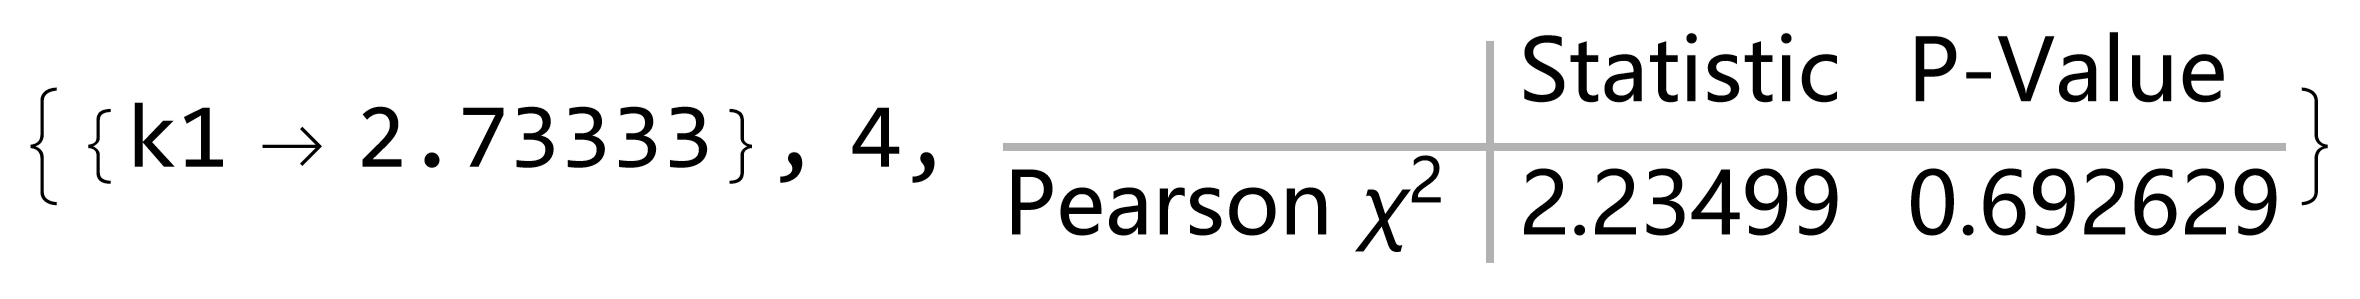
\includegraphics[width=0.6\linewidth]{poissonfit2.png}
\end{figure}

Hence, we can read off that $\widehat{k}_{2019}=2.73$. The null hypothesis is given by:
$$H_0:\text{ the number of fatal police shooting follows a Poisson distribution with parameter }\widehat{k}_{2019}=2.73$$

The $P$-value is $p=0.693$, which is extremely large. Hence, there is no reason to believe that the number of fatal police shooting is not Poisson distributed.

\subsubsection{Considering Pearson Criteria}
Considering the Pearson Criteria, we perform the following tests.
\paragraph{Step 1} Find an estimator for $k$.

The maximum-likelihood estimator for $\widehat{k}_{2019}$ is given by the sample mean.
\begin{align*}
\widehat{k}_{2019}
&=\overline{X}\\
&=\displaystyle\frac{1}{31+28+31}(8\times 0+16\times 1+22\times 2+\cdots+1\times 9)\\
&= 2.73
\end{align*}

\paragraph{Step 2} To apply the multinomial distribution, we calculate each element:
\begin{align*}
P[X=0] &=\displaystyle\frac{e^{-\widehat{k}}\widehat{k}^0}{0!}=0.0650023\\
P[X=1] &=\displaystyle\frac{e^{-\widehat{k}}\widehat{k}^1}{1!}=0.177673\\
P[X=2] &=\displaystyle\frac{e^{-\widehat{k}}\widehat{k}^2}{2!}=0.24282\\
&\cdots \qquad \cdots\\
P[X=9] &=1-P[X=1]-\cdots-P[X=8]=0.0021
\end{align*}

The results are shown as:
\begin{table}[!htbp]
  \centering
    \begin{tabular}{ccccccccccc}
    \hline
    Number of shoots & 0     & 1     & 2     & 3     & 4     & 5     & 6     & 7     & 8     & 9 \\
    \hline
    Category probabilities & 0.0650  & 0.1777  & 0.2428  & 0.2212  & 0.1512  & 0.0826  & 0.0376  & 0.0147  & 0.0050  & 0.0021  \\
    \hline
    \end{tabular}%
    \caption{The Category Probabilities}
\end{table}%

Consider the number of shoots as categories, the Category Random Variable is given by $(0.0650023, 0.177673,\\ 0.24282, 0.221236, 0.151178, 0.0826438, 0.0376488, 0.014701, 0.00502283, 0.00152545)$. 

\paragraph{Step 3} Upon this, we can calculate the expected frequencies by 
$$E_i=np_i=90p_i.$$

\newpage

The results are given by

\begin{table}[!htbp]
  \centering
    \begin{tabular}{ccccccccccc}
    \hline
    Categories & 0     & 1     & 2     & 3     & 4     & 5     & 6     & 7     & 8     & 9 \\
    \hline
    Expected Frequencies & 5.850  & 15.991  & 21.854  & 19.911  & 13.606  & 7.438  & 3.388  & 1.323  & 0.452  & 0.187  \\
    \hline
    \end{tabular}%
    \caption{The Expected Frequencies}
\end{table}%

\paragraph{Step 4} We noticed that the Pearson Criteria are not satisfied, because $E_{6-9}<5$ and $E_{8-9}<1$. We solve this problem by merging the last 4 categories to obtain:

\begin{table}[!htbp]
  \centering
    \begin{tabular}{ccccccccccc}
    \hline
    Categories & 0     & 1     & 2     & 3     & 4     & 5     & 6 \\
    \hline
    Expected Frequencies & 5.850  & 15.991  & 21.854  & 19.911  & 13.606  & 7.438  & 5.350  \\
    Observed Frequencies & 8.000  & 16.000  & 22.000  & 18.000  & 11.000  & 7.000  & 8.000  \\
    \hline
    \end{tabular}%
    \caption{The Merged Expected and Observed Frequencies}
\end{table}%

\paragraph{Step 5}
Then we can calculate the Pearson statistic:
$$\chi_{N-1-m}^2 = \sum^k_{i=1}\frac{(X_i-np_{i_0})^2}{np_{i_0}}=\sum^k_{i=1}\frac{(O_i-E_i)^2}{E_i}$$

The degrees of freedom is found by 
$$N-1-m=7-1-1=5,$$
and the statistic is found as
$$\chi_{5}^2 = 2.81152$$

\paragraph{Step 6} Fix $\alpha=0.05$, we test the null hypothesis with the $\chi^2_{0.05,5}=11.0705$. We found that
$$\chi_{5}^2 = 2.81152<11.0705=\chi^2_{0.05,5}$$

Hence we are unable to reject $H_0$.

\paragraph{Step 7} At last, we calculate the $P$-value of this test.
\begin{align*}
p &= P[\chi_5^2\ |\ H_0]\\
&\leq P[\chi^2\geq 2.81152] \\
&= 1-P[\chi^2\geq 2.81152]\\
&= 1-0.271\\
&=0.729
\end{align*}

The $P$-value is extremely large at $73\%$ level of significance, thus we fail to reject $H_0$.

The above calculations and tests proved that there is no evidence to believe that Poisson distribution fails describe the number of fatal police shooting in a day. Basically, Poisson distribution gives a good approximation.
\subsection{Bar Charts of Observed and Predicted Shooting Numbers}
The barcharts are plotted by \texttt{Mathematica}.

The observed numbers of fatal police shooting:
\begin{figure}[!htbp]
\centering
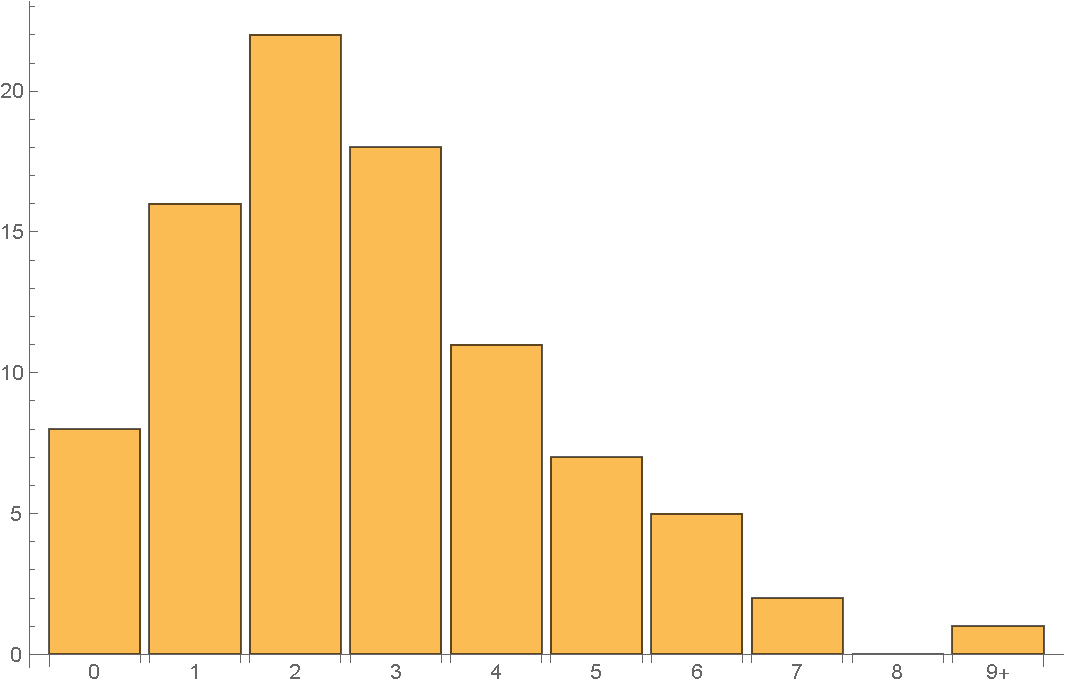
\includegraphics[width=0.8\linewidth]{observedbar2.pdf}
\caption{Observed Numbers of Fatal Police Shooting}
\end{figure}

The expected numbers of fatal police shooting:
\begin{figure}[!htbp]
\centering
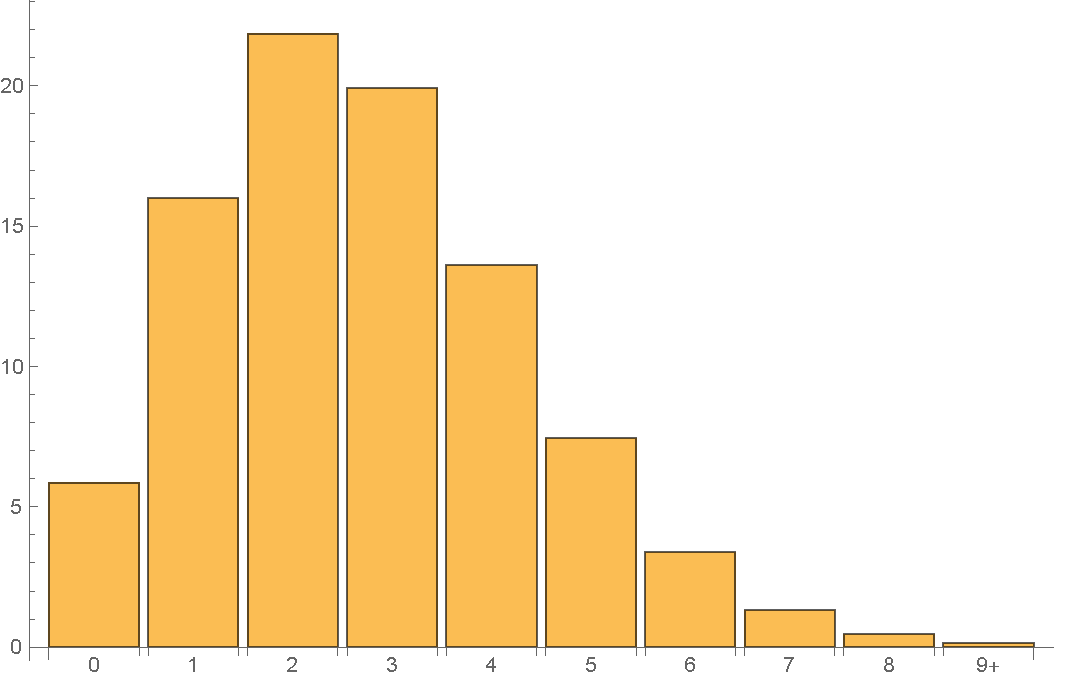
\includegraphics[width=0.8\linewidth]{expectedbar2.pdf}
\caption{Expected Numbers of Fatal Police Shooting}
\end{figure}

\newpage

\subsection{Prediction Interval for Number of Fatal Police Shooting}
\subsubsection{Derivation of Nelson's Formula}
The $100(1-\alpha)\%$ Nelson prediction interval we want to derive is retrieved from [5,(18)]:
$$[\lceil L \rceil,\lfloor U \rfloor] \text{ with } [L,U]=\widehat{Y}\pm z_{\alpha/2}\sqrt{m\widehat{Y}(\frac{1}{m}+\frac{1}{n})}$$

The proof is as follows.

\paragraph{Model Specification [5]}
Let $X$ be the total counts in a sample of size $n$ from a Poisson distribution with mean $\lambda$. Note that $X\sim$ Poisson$(n\lambda)$. Let $Y$ denote the future total counts that can be observed in a sample of size $m$ from the same Poisson distribution so that $Y\sim$ Poisson$(m\lambda)$. 

The conditional distribution of $X$,conditionally given $\displaystyle\frac{n}{n+m}$, is binomial with number of trials $s$ and the success probability $\displaystyle\frac{n}{n+m}$, binomial $(s,\displaystyle\frac{n}{n+m})$, and the conditional distribution of $Y$ given the sum $X+Y$ is binomial $(s,\displaystyle\frac{n}{n+m})$ [5].

\paragraph{Estimators [5,8]}
The estimators used in this formula nees specifications.
\begin{itemize}
\item The maximum-likelihood estimator $\widehat{\lambda}$ by the sample mean:
$$\widehat{\lambda} = \frac{X}{n}$$
\item The variance estimate $\widehat{\text{var}}(\widehat{Y}-Y)$:
$$\widehat{\text{var}}(\widehat{Y}-Y) = m^2\widehat{\lambda}(\frac{1}{m}+\frac{1}{n})$$
\item Estimate of essentially random $Y$ denoted as $\widehat{Y}$:
$$
\widehat{Y}=
\left\{
\begin{aligned}
&\frac{mX}{n}&=m\widehat{\lambda}\qquad & X=1,2,\cdots\\
&\frac{m}{2n}&  &X=0
\end{aligned}
\right.
$$

As $X$ assumes these values with positive probabilities, the coverage probabilities of the above PI are expected to be much smaller than the nominal level when $p$ of the binomial model is at the boundary $p=0$ and $p=n$ [8]. In Poisson model, when $p=0$ the approximation parameter $\lambda=np=0$ is at boundary as well. To overcome the poor coverage probabilities at the boundary, we can define $\widehat{\lambda}=\displaystyle\frac{0.5}{n}$ when $X=0$.
\end{itemize}

\paragraph{Statistic}
The statistic we use here the asymptotic result which is standard normal:
$$Z = \frac{m\widehat{\lambda}-Y}{\sqrt{\text{var}(m\widehat{\lambda}-Y)}}$$

Now, a $100(1-\alpha)\%$ prediction interval is given by:
\begin{align*}
1-\alpha &= P[-z_{\alpha/2} \leq Z \leq z_{\alpha/2}]\\
1-\alpha &= P[-z_{\alpha/2} \leq \frac{m\widehat{\lambda}-Y}{\sqrt{\text{var}(m\widehat{\lambda}-Y)}} \leq z_{\alpha/2}]\\
1-\alpha &= P[-z_{\alpha/2} \leq \frac{Y-m\widehat{\lambda}}{\sqrt{\text{var}(m\widehat{\lambda}-Y)}} \leq z_{\alpha/2}]\\
1-\alpha &= P[-z_{\alpha/2}\sqrt{\text{var}(m\widehat{\lambda}-Y)} \leq Y-m\widehat{\lambda} \leq z_{\alpha/2}\sqrt{\text{var}(m\widehat{\lambda}-Y)}]\\
1-\alpha &= P[-z_{\alpha/2}\sqrt{\text{var}(m\widehat{\lambda}-Y)} +m\widehat{\lambda} \leq Y \leq z_{\alpha/2}\sqrt{\text{var}(m\widehat{\lambda}-Y)}+m\widehat{\lambda}]\\
1-\alpha &= P[-z_{\alpha/2}\sqrt{m\widehat{Y}(\frac{1}{m}+\frac{1}{n})} +\widehat{Y} \leq Y \leq z_{\alpha/2}\sqrt{m\widehat{Y}(\frac{1}{m}+\frac{1}{n})}+\widehat{Y}]
\end{align*}

Hence, taking the ceiling of the lower prediction bound and the floor of the upper prediction bound for integer,
$$[\lceil L \rceil,\lfloor U \rfloor] \text{ with } [L,U]=\widehat{Y}\pm z_{\alpha/2}\sqrt{m\widehat{Y}(\frac{1}{m}+\frac{1}{n})}$$

\subsection{95$\%$ Prediction Intervals for 2019}
This formula allows us to find a prediction interval of the number of mass shootings in 2019. We first explain for each notations.

\begin{itemize}
\item $X$: the number of mass shootings between 2015 and 2018;
$$X=3943$$
\item $Y$: the number of mass shootings in 2019;
\item $n$: number of days between 2015 and 2018;
$$n=1461$$
\item $m$: the number of days considered in 2019;
\end{itemize}

Hence we can calculate $\widehat{Y}$ by
$$\widehat{Y}=\frac{mX}{n}=\frac{3943}{1461}m\approx 2.699m$$

Plug in the above data, we can find the prediction interval formula:
$$\lceil L \rceil = \widehat{Y}- z_{\alpha/2}\sqrt{m\widehat{Y}(\frac{1}{m}+\frac{1}{n})}$$
$$\lfloor U \rfloor = \widehat{Y}+ z_{\alpha/2}\sqrt{m\widehat{Y}(\frac{1}{m}+\frac{1}{n})}$$

The calculations are performed with $\alpha=0.05$, i.e. $z_{\alpha/2}=1.96$:
\begin{align*}
L
&= \widehat{Y}- z_{\alpha/2}\sqrt{m\widehat{Y}(\frac{1}{m}+\frac{1}{n})}\\
&= \frac{3943}{1461}m- 1.96\sqrt{\frac{3943}{1461}m^2(\frac{1}{m}+\frac{1}{1461})}\\
&= 2.69884m - 3.21991\sqrt{0.000684463m^2 + m}
\end{align*}
$$\lceil L \rceil = \lceil 2.69884m - 3.21991\sqrt{0.000684463m^2 + m} \rceil $$

\begin{align*}
U
&= \widehat{Y}+ z_{\alpha/2}\sqrt{m\widehat{Y}(\frac{1}{m}+\frac{1}{n})}\\
&= \frac{3943}{1461}m+ 1.96\sqrt{\frac{3943}{1461}m^2(\frac{1}{m}+\frac{1}{1461})}\\
&= 2.69884m + 3.21991\sqrt{0.000684463m^2 + m}
\end{align*}

$$\lfloor U \rfloor = \lfloor 2.69884m + 3.21991\sqrt{0.000684463m^2 + m} \rfloor $$

The plot is performed by \texttt{Mathematica}, and the figure is as follows.

For the whole year of 2019, the plot gives:
\begin{figure}[!htbp]
\centering
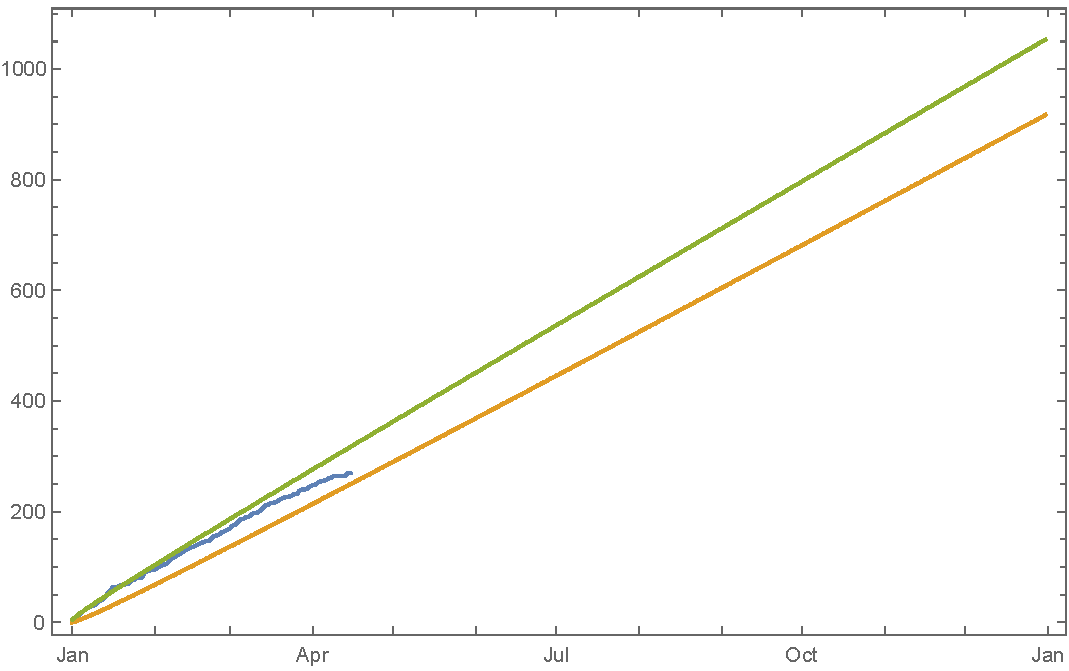
\includegraphics[width=1\linewidth]{predictall.pdf}
\caption{Prediction Interval and Updated Observed Data in 2019}
\end{figure}

\newpage

For the clearer view, we plot within the updated dates in 2019:
\begin{figure}[!htbp]
\centering
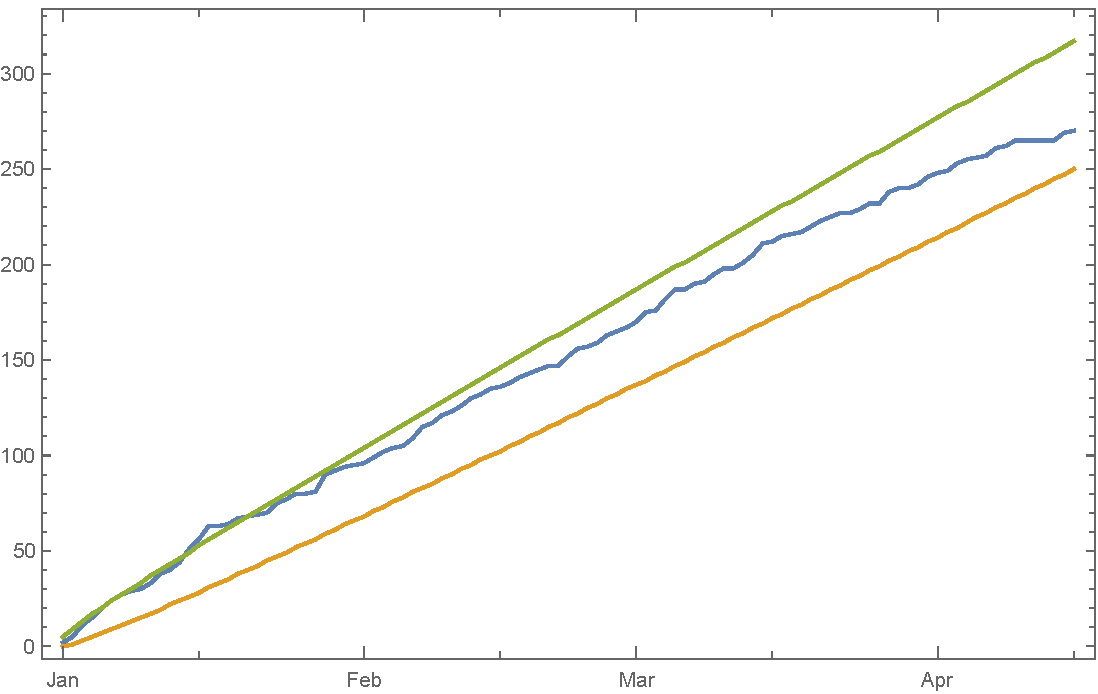
\includegraphics[width=1\linewidth]{predictapril.pdf}
\caption{Prediction Interval and Updated Observed Data before Apr. 15th, 2019}
\end{figure}

\paragraph{Comments}
With the graphs above, we basically conclude that the prediction interval gives a good prediction for the mass shooting in 2019, because the updated observed data generally lie within the band.

However, in the middle of January, the observed total shootings rise above the upper bound. This is statistically acceptable, because the confidence level is $95\%$.

We observed that at beginning, the observed data is closer to the upper bound. However, as the numbers go up, the observed data track back to the middle. This is because only wit large sample size, an approximate normal distribution is acceptable for the estimator of $k$.

\newpage

\section{Conclusion}
Analogous to \textit{London murders: a predictable pattern?} by David Spiegelhalter and Arthur Barnett, we develop our project based on the \textit{Database of Fatal Police Shootings} of the Washington Post. 

We first plot the everyday police shooting data between January 1$^{\text{st}}$, 2015 and December 31$^{\text{st}}$, 2015 to gain a straightforward impression. 

Then we test whether the occurrence of fatal police shooting from 2015 to 2018 follows a Poisson distribution, and our conclusion is that there's no evidence that it does not follow a Poisson distribution. 

Someone believes that weekday may influence the fatal police shooting rate, so we do a test based on Pearson statistic and draw a conclusion that the average number of shooting is independent of weekdays. 

Since we state that the police shooting from 2015 to 2018 follows a Poisson distribution, we are interested in the value of k. Our result is that there're at least 95\% possibility that k is in the interval [2.6146,2.7830]. With the training data from 2015 to 2018, we state the fatal police shooting follows a Poisson distribution. 

Then we use testing data from 2019 to test our statement. These data pass the test, which indicates that the data follows a Poisson distribution, and we calculate out the value of $\widehat { k } _ { 2019 }$ as 2.73. Finally, we get the 95\% prediction intervals for the number of mass shootings in 2019 based on the data of 2015 to 2018, which is shown in last section. 

In conclusion, we make use of fatal police shooting data from 2015 to 2018 to set a model and do prediction on 2019. That's a basic method to get preparation for what will happen in the future based on statistic. We hope this project can contribute a little for the analysis of fatal police shooting in US.



\newpage

\section{References}
\subsection{Works Cited}
[1] D. Spiegelhalter and A. Barnett. London murders: a predictable pattern? Significance, 6(1):5-8, 2009. \url{http://onlinelibrary.wiley.com/doi/10.1111/j.1740-9713.2009.00334.x/abstract}. [Online; accessed 15-April-2019].

[2] H. Hohberger. "ve401\uline{ }main.pdf"(2018). UMJI-SJTU, Shanghai. [Online; accessed 25-Feb-2019]. 

[3] DateHistogram. Wolfram. 2019. \url{https://reference.wolfram.com/language/ref/DateHistogram.html}.

[4] J. Tate, J. Jenkins, S. Rich, J. Muyskens, K. Elliott, T. Mellnik and A. Williams. How The Washington Post is examining police shootings in the United States. The Washington Post. July 7, 2016. \url{https://www.washingtonpost.com/national/how-the-washington-post-is-examining-police-shootings-in-the-united-states/2016/07/07/d9c52238-43ad-11e6-8856-f26de2537a9d_story.html?utm_term=.d357cd563cc4}. [Online; accessed 15-April-2019].

[5] K.Krishnamoorthy and J.Peng. Improved closed-form prediction intervals for binomial and Poisson distributions. Journal of Statistical Planning and Inference, 141(5):1709-1718, 2011. \url{http://www.sciencedirect.com/science/article/pii/S0378375810005215}. [Online; accessed 15-April-2019].

[6] Washington Post. Data-police-shootings. GitHub. \url{https://github.com/washingtonpost/data-police-shootings}. [Online; accessed 15-April-2019].

[7] Washington Post. Police Shootings 2019. \url{https://www.washingtonpost.com/graphics/2019/national/police-shootings-2019/?utm_term=.b08ecc24520c}. [Online; accessed 21-April-2019].

[8] H. Wang. 2008. Coverage probability of prediction intervals for discrete random variables. Computational Statistics and Data Analysis 53, 17-26.

[9] Wikipedia. Poisson Distribution, \textit{wikipedia}, the free encyclopedia, 2019. \url{https://en.wikipedia. org/wiki/Poisson_distribution} [Online; accessed 20-April-2019]. 
\section{Appendix}
\subsection{\texttt{Mathematica} and \texttt{Matlab} Codes}
\end{document}
